%%%%%%%%%%%%%%%%%%%%%%%%%%%%%%%%%%%%%%%%%
% Masters/Doctoral Thesis 
% LaTeX Template
% Version 1.43 (17/5/14)
%
% This template has been downloaded from:
% http://www.LaTeXTemplates.com
%
% Original authors:
% Steven Gunn 
% http://users.ecs.soton.ac.uk/srg/softwaretools/document/templates/
% and
% Sunil Patel
% http://www.sunilpatel.co.uk/thesis-template/
%
% License:
% CC BY-NC-SA 3.0 (http://creativecommons.org/licenses/by-nc-sa/3.0/)
%
% Note:
% Make sure to edit document variables in the Thesis.cls file
%
%%%%%%%%%%%%%%%%%%%%%%%%%%%%%%%%%%%%%%%%%

%----------------------------------------------------------------------------------------
%	PACKAGES AND OTHER DOCUMENT CONFIGURATIONS
%----------------------------------------------------------------------------------------

\documentclass[11pt, oneside]{Thesis} % The default font size and one-sided printing (no margin offsets)

\graphicspath{{Pictures/}} % Specifies the directory where pictures are stored

\usepackage[square, numbers, comma, sort&compress]{natbib} % Use the natbib reference package - read up on this to edit the reference style; if you want text (e.g. Smith et al., 2012) for the in-text references (instead of numbers), remove 'numbers' 

\usepackage{amsmath} % Mathe
\usepackage{mathtools} % Mathe
\usepackage{amsfonts} % Mathesymbole
\usepackage{calc}
\usepackage{url}
\usepackage{listings}
\usepackage{titlesec}

\usepackage{listings}
\usepackage{xcolor}

\titleformat
{\chapter} % command
[display] % shape
{\normalfont\Large\bfseries} % format
{Chapter \ \thechapter}
{0.5ex} % sep
{
    \rule{\textwidth}{1pt}
    \vspace{0ex}
    \centering
} % before-code
[
\vspace{-0.5ex}%
\rule{\textwidth}{0.3pt}
] % after-code

\lstdefinelanguage{scala}{
  morekeywords={abstract,case,catch,class,def,%
    do,else,extends,false,final,finally,%
    for,if,implicit,import,match,mixin,%
    new,null,object,override,package,%
    private,protected,requires,return,sealed,%
    super,this,throw,trait,true,try,%
    type,val,var,while,with,yield,specialized},
  otherkeywords={<-, =>,<\%,<:,>:,\#,@},
  sensitive=true,
  morecomment=[l]{//},
  morecomment=[n]{/*}{*/},
  morestring=[b]",
  morestring=[b]',
  morestring=[b]"""
}

\definecolor{ggray}{gray}{0.5}
\definecolor{Green}{HTML}{005500}
\definecolor{Blue}{HTML}{000099}

\renewcommand{\ttdefault}{pcr}
\lstset{frame=tb,
  language=scala,
  aboveskip=3mm,
  belowskip=0mm,
  showstringspaces=false,
  columns=flexible,
  %basicstyle={\footnotesize \ttfamily},
  basicstyle=\renewcommand{\baselinestretch}{0.95}\ttfamily,%
  %basicstyle=\LSTfont,
  numbers=none,
  numbersep=5pt,
  numberstyle=\tiny\color{Blue},
  keywordstyle=\color{Blue},
  commentstyle=\color{Green},
  frame=single,
  breaklines=true,
  breakatwhitespace=true
  tabsize=3
}


\hypersetup{urlcolor=blue, colorlinks=true} % Colors hyperlinks in blue - change to black if annoying
\title{\ttitle} % Defines the thesis title - don't touch this

\begin{document}

\frontmatter % Use roman page numbering style (i, ii, iii, iv...) for the pre-content pages

\setstretch{1.3} % Line spacing of 1.3

% Define the page headers using the FancyHdr package and set up for one-sided printing
\fancyhead{} % Clears all page headers and footers
\rhead{\thepage} % Sets the right side header to show the page number
\lhead{} % Clears the left side page header

\pagestyle{fancy} % Finally, use the "fancy" page style to implement the FancyHdr headers

\newcommand{\HRule}{\rule{\linewidth}{0.5mm}} % New command to make the lines in the title page

% PDF meta-data
\hypersetup{pdftitle={\ttitle}}
\hypersetup{pdfsubject=\subjectname}
\hypersetup{pdfauthor=\authornames}
\hypersetup{pdfkeywords=\keywordnames}               
            

%----------------------------------------------------------------------------------------
%	TITLE PAGE
%----------------------------------------------------------------------------------------

\begin{titlepage}
\begin{center}

\textsc{\LARGE \univname}\\[1.5cm] % University name
\textsc{\Large Master Thesis}\\[0.5cm] % Thesis type

\HRule \\[0.4cm] % Horizontal line
{\huge \bfseries \ttitle}\\[0.4cm] % Thesis title
\HRule \\[1.5cm] % Horizontal line
 
\begin{minipage}{0.4\textwidth}
\begin{flushleft} \large
\emph{Author:}\\
\href{http://www.johnsmith.com}{\authornames} % Author name - remove the \href bracket to remove the link
\end{flushleft}
\end{minipage}
\begin{minipage}{0.4\textwidth}
\begin{flushright} \large
\emph{Supervisor:} \\
\href{http://www.jamessmith.com}{\supname} % Supervisor name - remove the \href bracket to remove the link  
\end{flushright}
\end{minipage}\\[3cm]
 
\large \textit{A thesis submitted in fulfilment of the requirements\\ for the degree of \degreename}\\[0.3cm] % University requirement text
\textit{in the}\\[0.4cm]
\groupname\\\deptname\\[2cm] % Research group name and department name
 
{\large \today}\\[4cm] % Date
%\includegraphics{Logo} % University/department logo - uncomment to place it
 
\vfill
\end{center}

\end{titlepage}


%----------------------------------------------------------------------------------------
%	ABSTRACT PAGE
%----------------------------------------------------------------------------------------

\addtotoc{Abstract} % Add the "Abstract" page entry to the Contents

\abstract{\addtocontents{toc}{\vspace{1em}} % Add a gap in the Contents, for aesthetics

The Thesis Abstract is written here (and usually kept to just this page). The page is kept centered vertically so can expand into the blank space above the title too\ldots
}

\clearpage % Start a new page

%----------------------------------------------------------------------------------------
%	ACKNOWLEDGEMENTS
%----------------------------------------------------------------------------------------

%\setstretch{1.3} % Reset the line-spacing to 1.3 for body text (if it has changed)

%\acknowledgements{\addtocontents{toc}{\vspace{1em}} % Add a gap in the Contents, for aesthetics

%The acknowledgements and the people to thank go here, don't forget to include your project advisor\ldots
%}
%\clearpage % Start a new page

%----------------------------------------------------------------------------------------
%	LIST OF CONTENTS/FIGURES/TABLES PAGES
%----------------------------------------------------------------------------------------

\pagestyle{fancy} % The page style headers have been "empty" all this time, now use the "fancy" headers as defined before to bring them back

\lhead{\emph{Contents}} % Set the left side page header to "Contents"
\tableofcontents % Write out the Table of Contents

\lhead{\emph{List of Figures}} % Set the left side page header to "List of Figures"
\listoffigures % Write out the List of Figures

\lhead{\emph{List of Tables}} % Set the left side page header to "List of Tables"
\listoftables % Write out the List of Tables

%----------------------------------------------------------------------------------------
%	ABBREVIATIONS
%----------------------------------------------------------------------------------------

\clearpage % Start a new page

\setstretch{1.5} % Set the line spacing to 1.5, this makes the following tables easier to read

\lhead{\emph{Abbreviations}} % Set the left side page header to "Abbreviations"
\listofsymbols{ll} % Include a list of Abbreviations (a table of two columns)
{
\textbf{JVM} & \textbf{J}ava \textbf{V}irtual \textbf{M}achine \\
\textbf{JIT} & \textbf{J}ust \textbf{I}n \textbf{T}ime \\
\textbf{LHS} & \textbf{L}eft \textbf{H}and \textbf{S}ide \\
\textbf{RHS} & \textbf{R}igth \textbf{H}and \textbf{S}ide \\
\textbf{RB} & \textbf{R}adix \textbf{B}alanced \\
\textbf{RRB} & \textbf{R}elaxed \textbf{R}adix \textbf{B}alanced}

%----------------------------------------------------------------------------------------
%	PHYSICAL CONSTANTS/OTHER DEFINITIONS
%----------------------------------------------------------------------------------------

%\clearpage % Start a new page

%\lhead{\emph{Physical Constants}} % Set the left side page header to "Physical Constants"

%\listofconstants{lrcl} % Include a list of Physical Constants (a four column table)
%{
%Speed of Light & $c$ & $=$ & $2.997\ 924\ 58\times10^{8}\ \mbox{ms}^{-\mbox{s}}$ (exact)\\
% Constant Name & Symbol & = & Constant Value (with units) \\
%}

%----------------------------------------------------------------------------------------
%	SYMBOLS
%----------------------------------------------------------------------------------------

%\clearpage % Start a new page

%\lhead{\emph{Symbols}} % Set the left side page header to "Symbols"

%\listofnomenclature{lll} % Include a list of Symbols (a three column table)
%{
%$a$ & distance & m \\
%$P$ & power & W (Js$^{-1}$) \\
% Symbol & Name & Unit \\

%& & \\ % Gap to separate the Roman symbols from the Greek

%$\omega$ & angular frequency & rads$^{-1}$ \\
% Symbol & Name & Unit \\
%}

%----------------------------------------------------------------------------------------
%	DEDICATION
%----------------------------------------------------------------------------------------

%\setstretch{1.3} % Return the line spacing back to 1.3

%\pagestyle{empty} % Page style needs to be empty for this page

%\dedicatory{For/Dedicated to/To my\ldots} % Dedication text

%\addtocontents{toc}{\vspace{2em}} % Add a gap in the Contents, for aesthetics

%----------------------------------------------------------------------------------------
%	THESIS CONTENT - CHAPTERS
%----------------------------------------------------------------------------------------

\mainmatter % Begin numeric (1,2,3...) page numbering

\pagestyle{fancy} % Return the page headers back to the "fancy" style

% Include the chapters of the thesis as separate files from the Chapters folder
% Uncomment the lines as you write the chapters

I% Chapter Template

\chapter{Introduction} % Main chapter title

\label{Introduction} % Change X to a consecutive number; for referencing this chapter elsewhere, use \ref{ChapterX}

\lhead{Introduction} % Change X to a consecutive number; this is for the header on each page - perhaps a shortened title

%----------------------------------------------------------------------------------------
%	SECTION 1
%----------------------------------------------------------------------------------------

\section{Main Section 1}


%-----------------------------------
%	SUBSECTION 1
%-----------------------------------
\subsection{Subsection 1}


%-----------------------------------
%	SUBSECTION 2
%-----------------------------------

\subsection{Subsection 2}


%----------------------------------------------------------------------------------------
%	SECTION 2
%----------------------------------------------------------------------------------------

\section{Main Section 2}

I% Chapter Template

\chapter{Vector Structure} % Main chapter title

\label{VectorStructure} % Change X to a consecutive number; for referencing this chapter elsewhere, use \ref{ChapterX}

\lhead{Vector Structure. \emph{Vector Structure}} % Change X to a consecutive number; this is for the header on each page - perhaps a shortened title

%----------------------------------------------------------------------------------------
%	SECTION - Radix Balanced Vectors
%----------------------------------------------------------------------------------------

\section{Radix Balanced Vectors}

%-----------------------------------
%	SUBSECTION - Tree structure
%-----------------------------------

\subsection{Tree structure}
% describe tree: balancing, filling, block sizes
% why structure helps with operations implementation 
% hint why radix?  


\begin{figure}[h!]
  \centering
  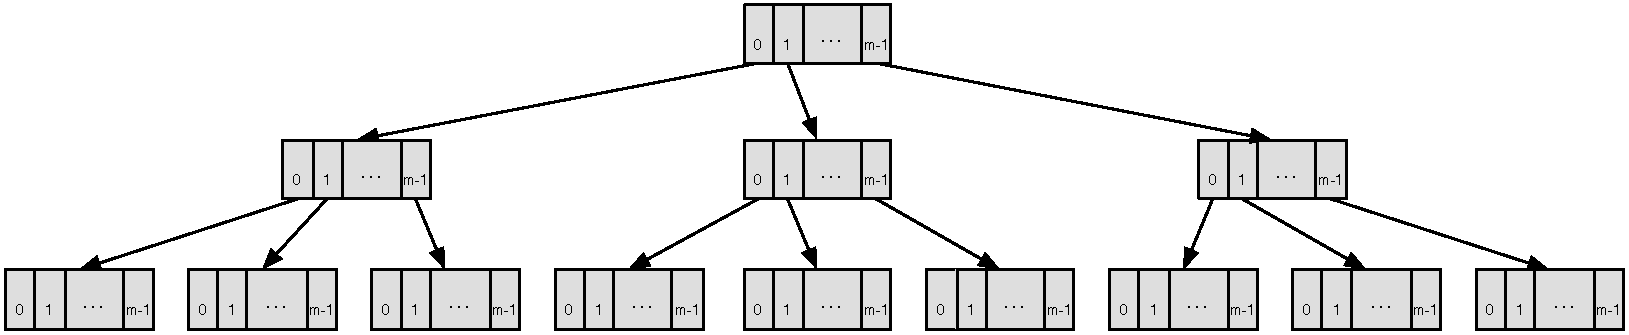
\includegraphics[width=\textwidth]{Figures/Radix_Balanced}
  \label{badix_balanced}
  \caption{Radix Balanced Tree Structure}
\end{figure}



%-----------------------------------
%	SUBSECTION - Operations
%-----------------------------------
\subsection{Operations}
% List core operations
% naive implementation just as high level guide
% Hint of displays and transient states


%-----------------------------------
%	SUBSUBSECTION - Apply
%-----------------------------------

\subsubsection{Apply}
% used in head and last
% performance log_32(n), hint of displays

\begin{lstlisting}[frame=single]
def apply(index: Int): A = {
  def getElem(node: Array[AnyRef], depth: Int): A = {
    val indexInNode = // get subindex
    if(depth == 1) node(indexInNode)
    else getElem(node(indexInNode), depth-1) 
  }
  getElem(vectorRoot, vectorDepth)
}
\end{lstlisting}

%-----------------------------------
%	SUBSUBSECTION - Updated
%-----------------------------------

\subsubsection{Updated}
% base implementation needs to update the whole branch
% with transient states, local updates can be amortised

\begin{lstlisting}[frame=single]
def updated(index: Int, elem: A) = {
  def updatedNode(node: Array[AnyRef], depth: Int) = {
    val indexInNode = // compute index
    val copy = clone(node)
    if(depth == 1) {
      copy(indexInNode) = elem
    } else {
      copy(indexInNode) = 
        updatedNode(node(indexInNode), depth-1)
    }
    copy
  }
  new Vector(updatedNode(vectorRoot, vectorDepth), ...)
}
\end{lstlisting}

%-----------------------------------
%	SUBSUBSECTION - Additions
%-----------------------------------

\subsubsection{Additions}

\paragraph{Append}
% base implementation needs to update the whole branch
% performance log_32(n), hint of transient to amortise consecutive appends are amortised

\paragraph{Prepend}
% base implementation needs to update the whole branch
% shift top and start index
% performance log_32(n), hint of transient to amortise consecutive appends are amortised

\paragraph{Concatenation and Insert}
% describe high level implementation in vector
%% describe branch rebalancing 
% performance O(n)


%-----------------------------------
%	SUBSUBSECTION - Splits
%-----------------------------------

\subsubsection{Splits}
% used in tail, init, take, takeRight, drop, dropRight
% describe implementation in vector
% performance log_32(n) 


%----------------------------------------------------------------------------------------
%	SECTION - Parallel Vectors
%----------------------------------------------------------------------------------------

\section{Parallel Vectors}
% why are  parallel vector useful
% how are they paralellized (wraps an vector)
% why do they suffer performance wise (no efficient concat)
% fork-join pool

%-----------------------------------
%	SUBSUBSECTION - Splitter
%-----------------------------------

\subsection{Splitter (Iterator)}
% split into half 
To divide the work into tasks for thread pool, a splitter is used to iterate over all elements of the collection. Splitters are a special kind of iterator that can be split at any time into some partition of the remaining elements. In the case of sequences the splitter should retain the original order. The most common implementation consists in dividing the remaining elements into two half. 

The current implementation of the immutable parallel  vector \cite{scalaParVector211}  uses the common division into 2 parts for it splitter. The drop and take operations are used divide the vector for the two new splitters.

%-----------------------------------
%	SUBSUBSECTION - Combiner
%-----------------------------------

\subsection{Combiner (Builder)}
% lazy combiner
Combiners are used to merge the results from different tasks (in methods like map, filter, collect, ...) into the new collection. Combiners are a special kind of builder that is able to merge to partial results efficiently. When it's impossible to implement efficient combination operation, usually a lazy combiner is used. The lazy combiner is one keeps all the it's sub-combiners in an array buffer and only when the end result is needed they are combined. This is a fairly efficient implementation but does not take full advantage of parallelism. 

The current implementation of the immutable parallel vector \cite{scalaParVector211} use the lazy approach because of it's inefficient concatenation operation. One of the consequences of this is that the parallel operations will always be bounded by this sequential combination of elements, which can be beaten by the sequential version in many cases.
 

%----------------------------------------------------------------------------------------
%	SECTION - Relaxed Radix Balanced Vectors
%----------------------------------------------------------------------------------------

\section{Relaxed Radix Balanced Vectors}

%-----------------------------------
%	SUBSECTION - Tree structure
%-----------------------------------

\subsection{Relaxed Tree structure}
% describe tree: balancing, filling, block sizes
% describe sizes array and where it is kept (change from left to right for indexing simplification)
% mention size of nodes and null sizes
% unbalanced trees can only be generated by concatenation, and splits

\begin{figure}[h!]
  \centering
  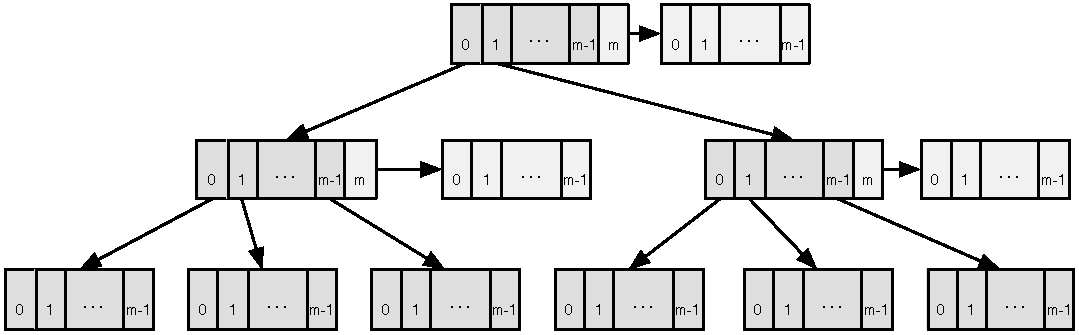
\includegraphics[width=\textwidth]{Figures/Relaxed_Radix_balanced}
  \label{Relaxed_Radix_balanced}
  \caption{Radix Balanced Tree}
\end{figure}

\begin{figure}[h!]
  \centering
  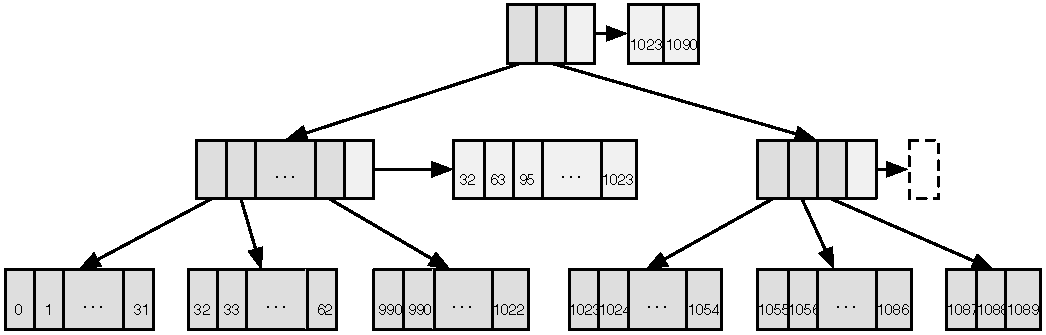
\includegraphics[width=\textwidth]{Figures/Relaxed_radix_example}
  \label{Relaxed_radix_example}
  \caption{Relaxed radix example}
\end{figure}

%-----------------------------------
%	SUBSECTION - Operations
%-----------------------------------
\subsection{Relaxed Operations}
% describe how the implementation uses relaxed radix when necessary and uses radix based operation when possible

%-----------------------------------
%	SUBSUBSECTION - Apply
%-----------------------------------

\subsubsection{Apply (get element at index)}
% describe the way to get the node indices in an unbalanced node


%-----------------------------------
%	SUBSUBSECTION - Updated
%-----------------------------------

\subsubsection{Updated}
% doesn't change much, the sizes do not need to be updated, they jus need to be copied. Going to the correct position still may needs to access the sizes.

%-----------------------------------
%	SUBSUBSECTION - Additions
%-----------------------------------

\subsubsection{Additions}

%-----------------------------------
\paragraph{Append}
% difference is that the the sizes may need to be updated
% performance log_32(n), remind hint of transient to amortise consecutive appends are amortised

\paragraph{Prepend}
% describe different implementation
% hint the 


%-----------------------------------
\paragraph{Concatenation}
% describe high level implementation in rrbvector
%% describe branch rebalancing 
% performance log_32(n)

\begin{figure}[h!]
  \centering
  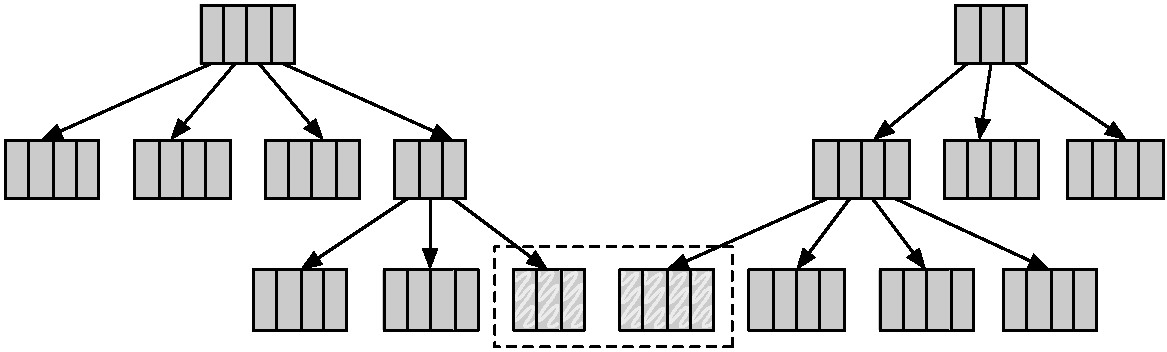
\includegraphics[width=\textwidth]{Figures/Concat0.pdf}
  \label{Concat0Benchmarks}
  \caption{Concatenation example with blocks of size 4: Rebalancing level 0}
\end{figure}

\begin{figure}[h!]
  \centering
  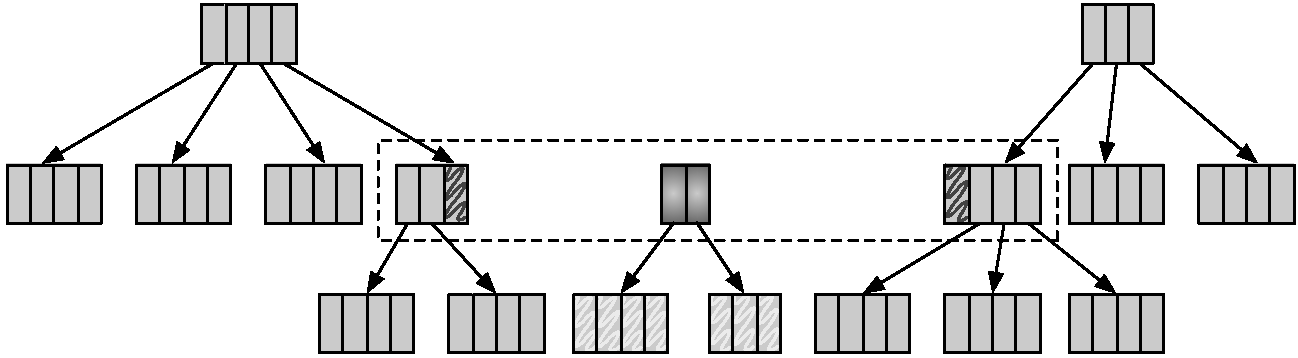
\includegraphics[width=\textwidth]{Figures/Concat1.pdf}
  \label{Concat1Benchmarks}
  \caption{Concatenation example with blocks of size 4: Rebalancing level 1}
\end{figure}

\begin{figure}[h!]
  \centering
  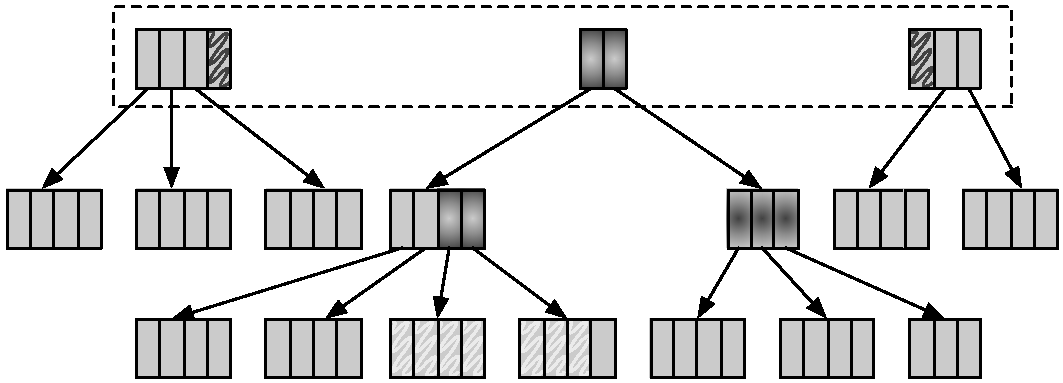
\includegraphics[width=\textwidth]{Figures/Concat2.pdf}
  \label{Concat2Benchmarks}
  \caption{Concatenation example with blocks of size 4: Rebalancing level 2}
\end{figure}

\begin{figure}[h!]
  \centering
  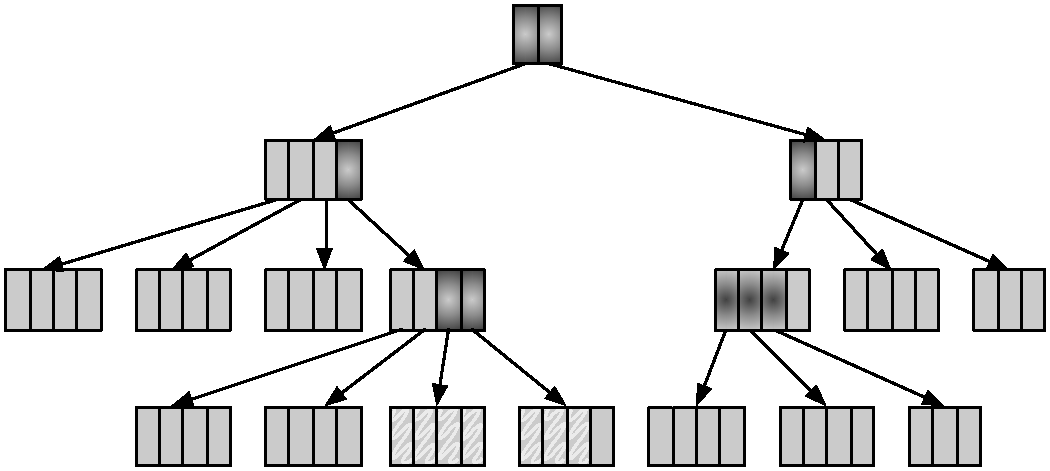
\includegraphics[width=\textwidth]{Figures/Concat3.pdf}
  \label{Concat3Benchmarks}
  \caption{Concatenation example with blocks of size 4: Rebalancing level 3}
\end{figure}


%-----------------------------------
\paragraph{Insert}
% new operation
% describe simple implementation using split and concat 
% performance log_32 (from split + concat)
% hint at possible optimization by inserting directly and using transient states (take advantage of locality)



%-----------------------------------
%	SUBSUBSECTION - Splits
%-----------------------------------

\subsubsection{Splits}
% used in tail, init, take, takeRight, drop, dropRight
% describe difference between the implementation (null and shift vs. cut and update size)

%-----------------------------------
%	SUBSUBSECTION - Splits
%-----------------------------------

\subsubsection{Parallel Vector}
% Combine: trivial expansion from builder
%% heuristic: try to construct balanced trees 
% Split into subtrees two, take the nearest power of 32 to the half



I% Chapter Template

\chapter{Optimizations} % Main chapter title

\label{Optimizations} % Change X to a consecutive number; for referencing this chapter elsewhere, use \ref{ChapterX}

\lhead{Optimizations. \emph{Optimizations}} % Change X to a consecutive number; this is for the header on each page - perhaps a shortened title

%----------------------------------------------------------------------------------------
%	SECTION - Where does time go?
%----------------------------------------------------------------------------------------

\section{Where is time spent?}

%-----------------------------------
%	SUBSECTION 1
%-----------------------------------

\subsection{Arrays}
% array creation, copy
Most of the memory used in the vector data structure is composed of arrays. The three key operations used on these arrays: array creation, array update and array access. The arrays are used as immutable arrays, as such the update operations are only allowed when the array is initialised. This also implies that each time there is a modification on some part of an array, a new array must be created and all the old elements copied. 

% size of array argument
The size of the array will affect the performance of the vector. With larger blocks the access times will be reduced because the depth of the tree will decrease. But, on the other hand, increasing the size of the block will make slow down the update operations. This is a direct consequence of the need to copy the entire array for a single update.


%-----------------------------------
%	SUBSECTION 2
%-----------------------------------

\subsection{Computing indices}
\label{ComputingIndices}

Computing the indices in each node while traversing or modifying the vector is key in performance. This performances is gained by using low level binary computations on the indices in the case where the tree is balanced. And, using precomputed sizes in the case where the balance is relaxed.

%-----------------------------------
\paragraph{Radix}
% Explain how to compute them
Assuming that the tree is full, elements are fetched from the tree using radix search on the index. As each node has a branching of 32, the index can be split bitwise in blocks of 5 ($2^5 = 32$) and used to know the path that must be taken from the root down to the element. The indices at each level $L$ can be computed with $(index >> (5 \cdot L)) \& 31$. For example the index 526843 would be:
\[
 526843 = 00
   	 \underbracket[0.2pt][4pt]{00000}_{\text{0}}
   	 \underbracket[0.2pt][4pt]{00000}_{\text{0}}
  	 \underbracket[0.2pt][4pt]{10000}_{\text{16}}
 	 \underbracket[0.2pt][4pt]{00010}_{\text{2}}
	 \underbracket[0.2pt][4pt]{01111}_{\text{15}}
     \underbracket[0.2pt][4pt]{11011}_{\text{27}}
\]

\begin{lstlisting}[frame=single]
def getSubIndex(indexInTree: Int, level: Int): Int = 
  (index >> (5*level)) & 31
\end{lstlisting}

% how to generalise
This scheme can be generalised to any block size $m$ where $m=2^i$ for $0 < i \leq 31$. The formula would be $(index >> (m \cdot L)) \& ((1<<m)-1)$. It is also possible to generalise for other values of $m$ using the modulo, division and power operations. In that case the formula would become $(index / (m^L)) \% m$. This last generalisation is not used because it reduces sightly the performance and it complicates other index manipulations. 

\begin{figure}[h!]
  \centering
  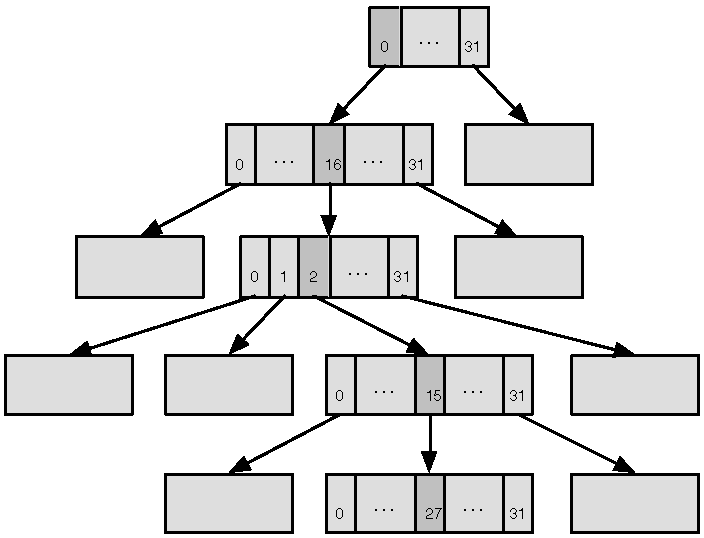
\includegraphics[width=0.5\textwidth]{Figures/Radix_Balanced_index_example}
  \caption{Accessing element at index 526843 in a tree of depth 5. Empty nodes represent collapses subtrees.}
  \label{radix_balanced_index_example}
\end{figure}

%-----------------------------------
\paragraph{Relaxing the Radix}
% Explain how to compute them 
When the tree is relaxed it is not possible to know the subindices from index. That is why we keep the sizes array in the unbalanced nodes. This array keeps the accumulated sizes to make the computation of subindices as trivial as possible. The subindex is the same as the first index in the sizes array where $index < sizes[subindex]$. The simplest way to find this subindex is by a linearly scanning the array. 

\begin{lstlisting}[frame=single]
def getSubIndex(sizes: Array[Int], indexInTree: Int): Int = {
  var is = 0
  while (sizes(is) <= indexInTree)
    is += 1
  is
}
\end{lstlisting}

% linear vs binary search
For small arrays (like blocks of size 32) this will take be faster than a binary search because it takes advantage of the cache lines. If we would consider using bigger block sizes it would be better to use a hybrid between binary and linear search.

% fallback to radix
To traverse the tree down to the leaf where the index is, the subindices are computed from the sizes as long as the tree node is unbalanced. If the node is balanced, then the more efficient radix based method is used from there to the leaf. To avoid the need of accessing and scanning an additional array in each level.


%-----------------------------------
%	SUBSECTION 3
%-----------------------------------

\subsection{Abstractions}
% function calls
% generic code vs specialized code
% expanded code 
% example with simple expanded get operation (show expansion and specialisation)


%----------------------------------------------------------------------------------------
%	SECTION - Displays
%----------------------------------------------------------------------------------------

\section{Displays}
\label{sec:Displays}
% describe display fields in vector object
As base for optimizations, the vector object keeps a set of fields to track one branch of the tree. They are named with using the level number from 0 up to the maximum possible level. In the case of blocks of size 32 the maximum level used is 5 \footnote{As in practice, only the 30 bits of the index are used.}, they are allocated by default and nulled if the tree if shallower. The highest non null display is and replaces the root field. All displays bellow the root are never null. This implies that the vector will always be focused on some branch.

\begin{figure}[h!]
  \centering
  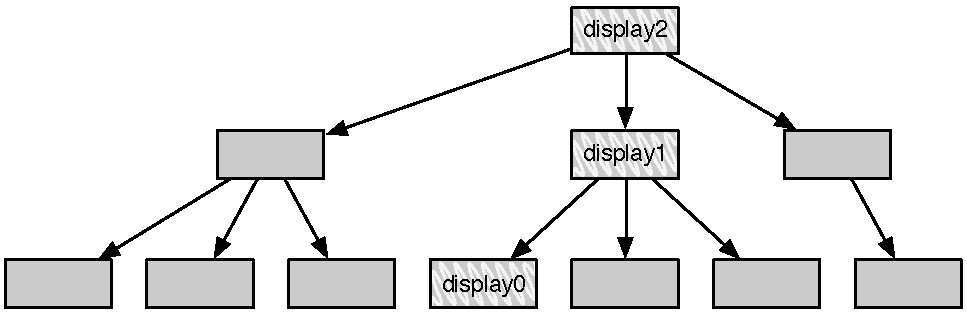
\includegraphics[width=0.8\textwidth]{Figures/Displays}
  \label{Displays}
  \caption{Displays}
\end{figure}

% describe the focus field
To know on which branch the vector is focused there is also a \texttt{focus} field with an index. This index is the index of any element in the current \texttt{display0}. This index represents the radix indexing scheme of node subindices described in \ref{ComputingIndices}.

% immutability of displays
To follow the simple implementations scheme of immutable objects in concurrent contexts, the focus is also immutable. Therefore each vector object will have a single focused branch during its existence\footnote{The display focus may change during the initialisation of the object as optimisation of some methods}. Each method that creates a new vector must decide which focus to set. 

%-----------------------------------
%	SUBSECTION As cache
%-----------------------------------

\subsection{As cache}
% used to access some elements directly from the smaller subtrees (XOR)
One of the uses of the displays is as a cached branch. If the same leaf node is used in the following operation, there is no need for vertical tree traversal which is key to amortize operation to constant time. In the case another branch in needed, then it can be fetched from the lowest common node of the two branches. 

% xor
To know the which is the level of the lowest common node in a vector of block size $2^m$ (for some consistent $m$), only the \texttt{focus} index and the index being fetched are needed. The operation $index \veebar focus$ will return a number is bounded to the maximum number of elements in a tree of that level. The actual level can be extracted with some if statements. This operation bounded by the same number of operations that will be needed to traverse the tree back down through the new branch.

\begin{lstlisting}[frame=single]
def getLowestCommonLevel(index: Int, focus: Int): Int = {
  val xor = index ^ focus
  if (xor < 32 /*(1<<5)*/ ) 0
  else if (xor < 1024 /*(1<<10)*/ ) 1
  else if (xor < 32768 /*(1<<15)*/ ) 2
  ...
  else 5
}
\end{lstlisting}

% keeping relevant branch for next operations
When deciding which will be the focused branch of a new vector two heuristics are used for this: If there was an update operation on some branch where that operations could be used again, that branch is used as focus. If the first one cant be applied, the display is set to the first element as this helps key collection operations such as \texttt{iterator}.

%-----------------------------------
%	SUBSECTION  For transient states
%-----------------------------------

\subsection{For transient states}
% operation: append, prepend, update
Transient states is the key optimisation to get append, prepend and update to amortized constant time. It consists in decoupling the tree by creating an equivalent tree that does not contain the edges on the current focused branch. The information missing in the edges of the tree is represented and can be reconstructed from the displays. In the current version of the collections vector \cite{scalaVector211} this state is identified by the \texttt{dirty} flag.

\begin{figure}[h!]
  \centering
  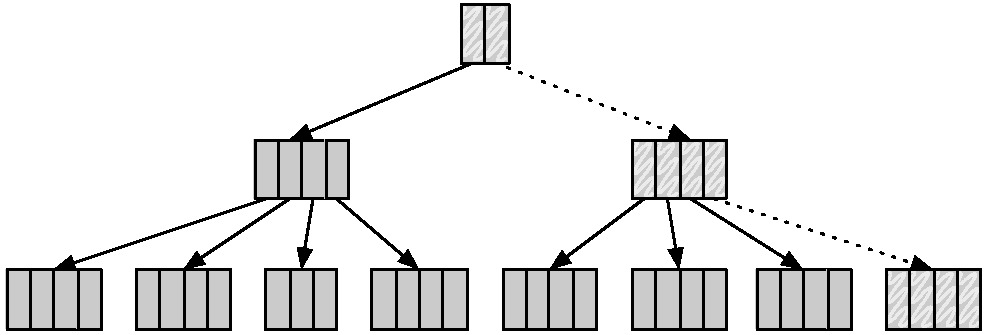
\includegraphics[width=\textwidth]{Figures/Transient_state}
  \label{Transient_state}
  \caption{Transient Tree with current focus displays marked in white and striped nulled edges.}
\end{figure}

% transient states are used to amortized operations
Without transient states when some update is done on a leaf, all the branch must be updated. On the other hand, if the state is transient, it is possible to update only the subtree affected by the change. In the case of updates on the same leaf, only the leaf must be updated. When appending or prepending, $\frac{31}{32}$ operations must only update the leaf, then $\frac{31}{1024}$ need to update two levels of the tree and so on. These operations will thus be amortized to constant ($\sum_{k=1}^{\infty} \frac{k*31}{32^k} = \frac{32}{31}$ block updates per operation) time if they are executed in succession.

% normailization
There is a cost associated to the transformation from normal state to transient state and back. This cost is equivalent to one update of the focused branch. The transient state operations only start gaining performance on the normal ones after 3 consecutive operations. With 2 consecutive operations they are matched and with 1 there is a loss of performance.


%-----------------------------------
%	SUBSECTION  Relaxing the Displays
%-----------------------------------

\subsection{Relaxing the Displays}
% describe fundamental difference in the focus (focused on balanced subtree)
When relaxing the tree balance it is also necessary to relax the displays. This is mainly due to the loss of a simple way to compute the lowest common node on unbalanced trees. Computing the node requires now the additional sizes information located in each unbalanced node. As such it is necessary to access the nodes to be abel to compute the lowest common node, and there is a loss in performance due to increased memory accesses. 

% describe focus start, focus end and focus (focus relaxed)
To still take advantage of efficient operations on balanced trees, the display is relaxed to be focused on a branch of some balanced subtree\footnote{A fully balanced tree will be itself the balanced subtree, as such it will always use the more performant operations.}. To keep track of this subtree there are three additional fields: \texttt{focusStart} that represents start index of the current focused subtree, \texttt{focusEnd} that represents the end index of the subtree and \texttt{focusDepth} that sets  height of the focused subtree\footnote{As an optimisation, the \texttt{focus} field is split into the part corresponding to the subtree and the part that represents the indices of the displays that are unbalanced.}. The operations that can take advantage of the the efficient display operations will check if the index is in the subtree index range and invoke the efficient operation. If not, it will invoke the relaxed version of the operation, that starts from the root of the tree.

% describe how fetching elements change
For example, the code for \texttt{getElement} would become:
\begin{lstlisting}[frame=single]
def getElement(index: Int): A = {
  if (focusStart <= index && index < focusEnd) 
    getElementFromDisplay(index - focusStart)
  else if (0 <= index && index < endIndex) 
    getElementFromRoot(index)    
  else 
    throw new IndexOutOfBoundsException(index)
}
\end{lstlisting}

This \texttt{getElement} on the unbalanced subtrees of figure \ref{Balanced_subtrees}  would use the \texttt{getElementFromDisplay} to fetch elements in \texttt{display0} directly from it and fetch elements from nodes (1.1) and (1.2) from \texttt{display1}. The rest is fetched from the root using \texttt{getElementFromRoot}.

\begin{figure}[h!]
  \centering
  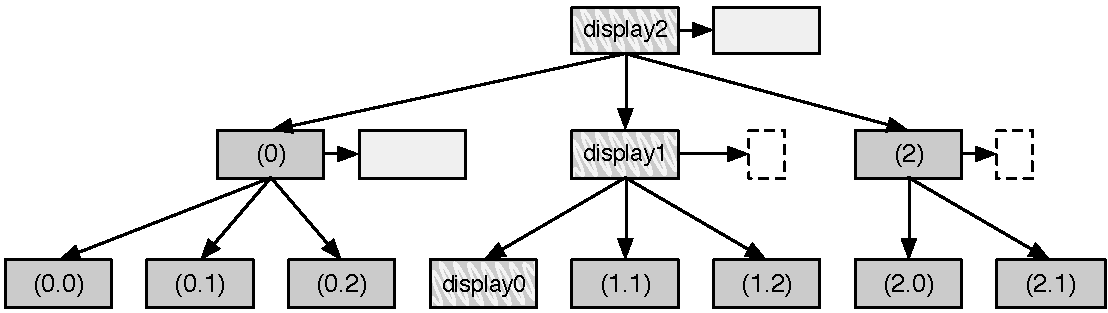
\includegraphics[width=\textwidth]{Figures/Balanced_subtrees}
  \caption{Relaxed Radix Balanced Tree with a focus on a balanced subtree rooted of \texttt{display1}. Light grey boxes represent unbalanced nodes sizes.}
  \label{Balanced_subtrees}
\end{figure}


%----------------------------------------------------------------------------------------
%	SECTION - Builder
%----------------------------------------------------------------------------------------

\section{Builder}
% use of mutable tree 
% avoid creation unnecessary arrays


%-----------------------------------
\paragraph{Relaxing the Builder}
% same base implementation for +=
% addition of accumulator for  ++= 



%----------------------------------------------------------------------------------------
%	SECTION - Iterator
%----------------------------------------------------------------------------------------

\section{Iterator}
% efficient tree traversal vs iteration by index
% avoid re-traversing vertically the tree from the root

%-----------------------------------
\paragraph{Relaxing the Iterator}
% same implementation within a balanced subtree
% refocus from root to iterate between balanced subtrees







 
I% Chapter Template

\chapter{Performance} % Main chapter title

\label{Performance} % Change X to a consecutive number; for referencing this chapter elsewhere, use \ref{ChapterX}

\lhead{Performance. \emph{Performance in practice and Benchmarks}} % Change X to a consecutive number; this is for the header on each page - perhaps a shortened title


%----------------------------------------------------------------------------------------
%	SECTION In practice: Running on JVM
%----------------------------------------------------------------------------------------
\section{In practice: Running on JVM}
\label{InPractice}
% code interpreted vs compiled
\color{red} TODO \color{black}

% GC and memory allocations
\color{red} TODO \color{black}
% memory access and caches

\subsection{Arrays}
% system arraycopy primitive
\color{red} TODO \color{black}

%-----------------------------------
%	SUBSECTION Cost of Abstraction
%-----------------------------------
\subsection{Cost of Abstraction and JIT Inline}
% cost of function invokation
% code compiled (inlined if hot)
% aim to make all critical methods 35< bytes
\color{red} TODO \color{black}



%----------------------------------------------------------------------------------------
%	SECTION Scalameter
%----------------------------------------------------------------------------------------
\section{Measuring performance}
% Scalameter
% warmup to JIT inline
% using vectors that do not fill perfectly the last branch to avoid trivial cases (that would be faster but do not show the average of the operation)

\color{red} TODO \color{black}

%----------------------------------------------------------------------------------------
%	SECTION Generators
%----------------------------------------------------------------------------------------
\section{Implementation Generators}
% block sizes
% concat implementation
% balanced, a bit unbalanced and extremely unbalanced

\color{red} TODO \color{black}

%----------------------------------------------------------------------------------------
%	SECTION Benchmarks
%----------------------------------------------------------------------------------------
\section{Benchmarks}
% describe the the different benchmark types 
%% differences between implementation (vector vs rrbvector)
%% differences between unbalances
%% differences between block sizes
%% differences between concatenation rebalancing method
\color{red} TODO \color{black}

%-----------------------------------
%	SUBSECTION Apply
%-----------------------------------
\subsection{Apply}
% describe the benchmark function
% compare expectation with results
% explain the upper bound
% explain apparently incoherent results
\color{red} TODO \color{black}

\begin{figure}[h!]
  \centering
  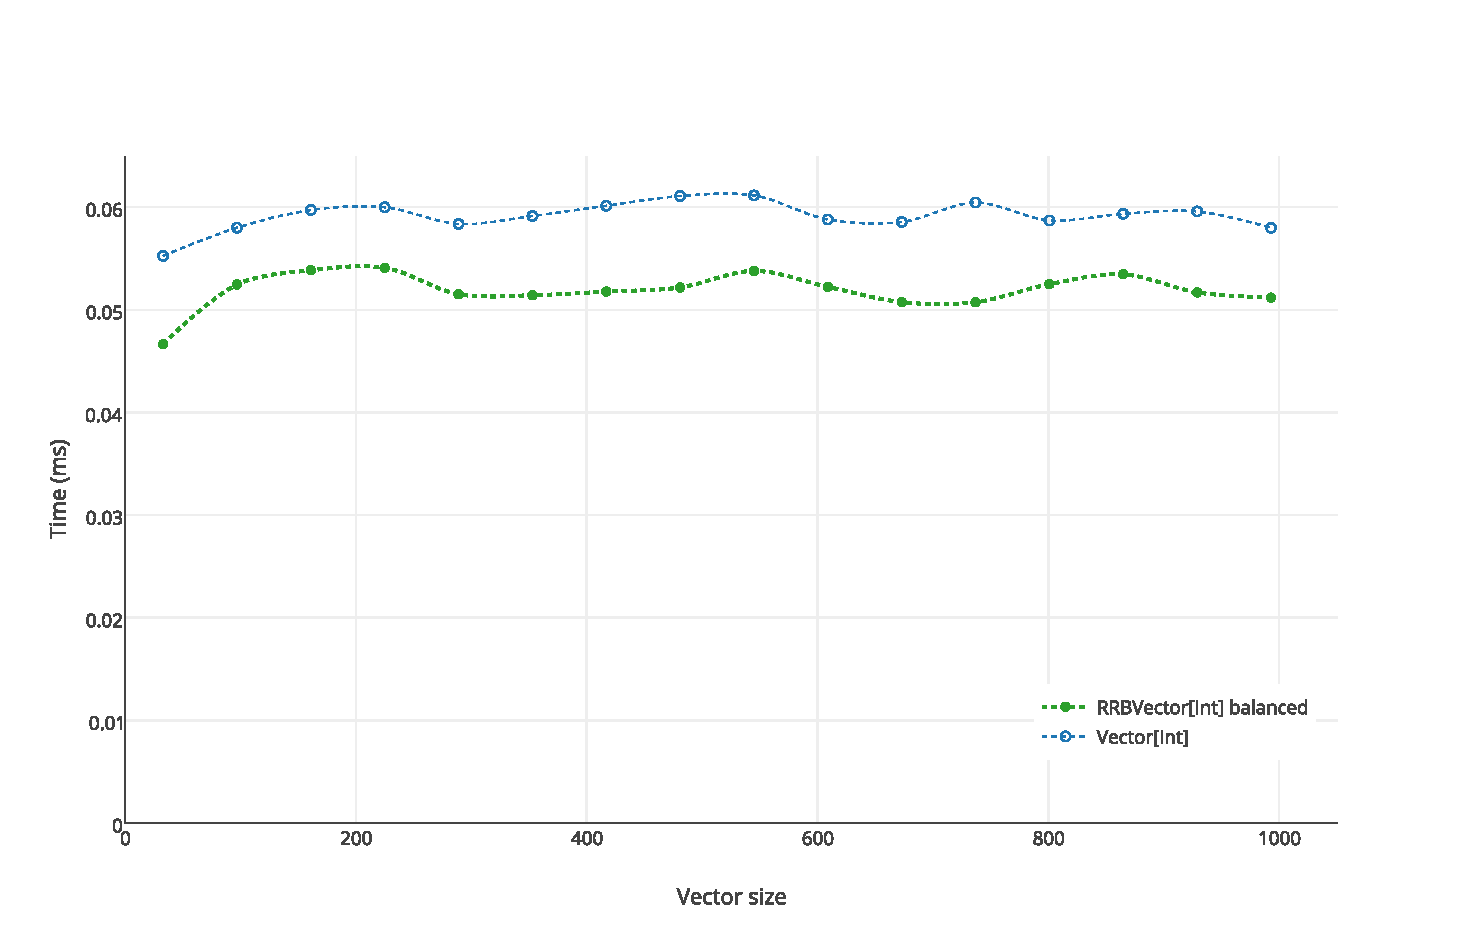
\includegraphics[width=\textwidth]{Benchmarks/Apply_2.pdf}
  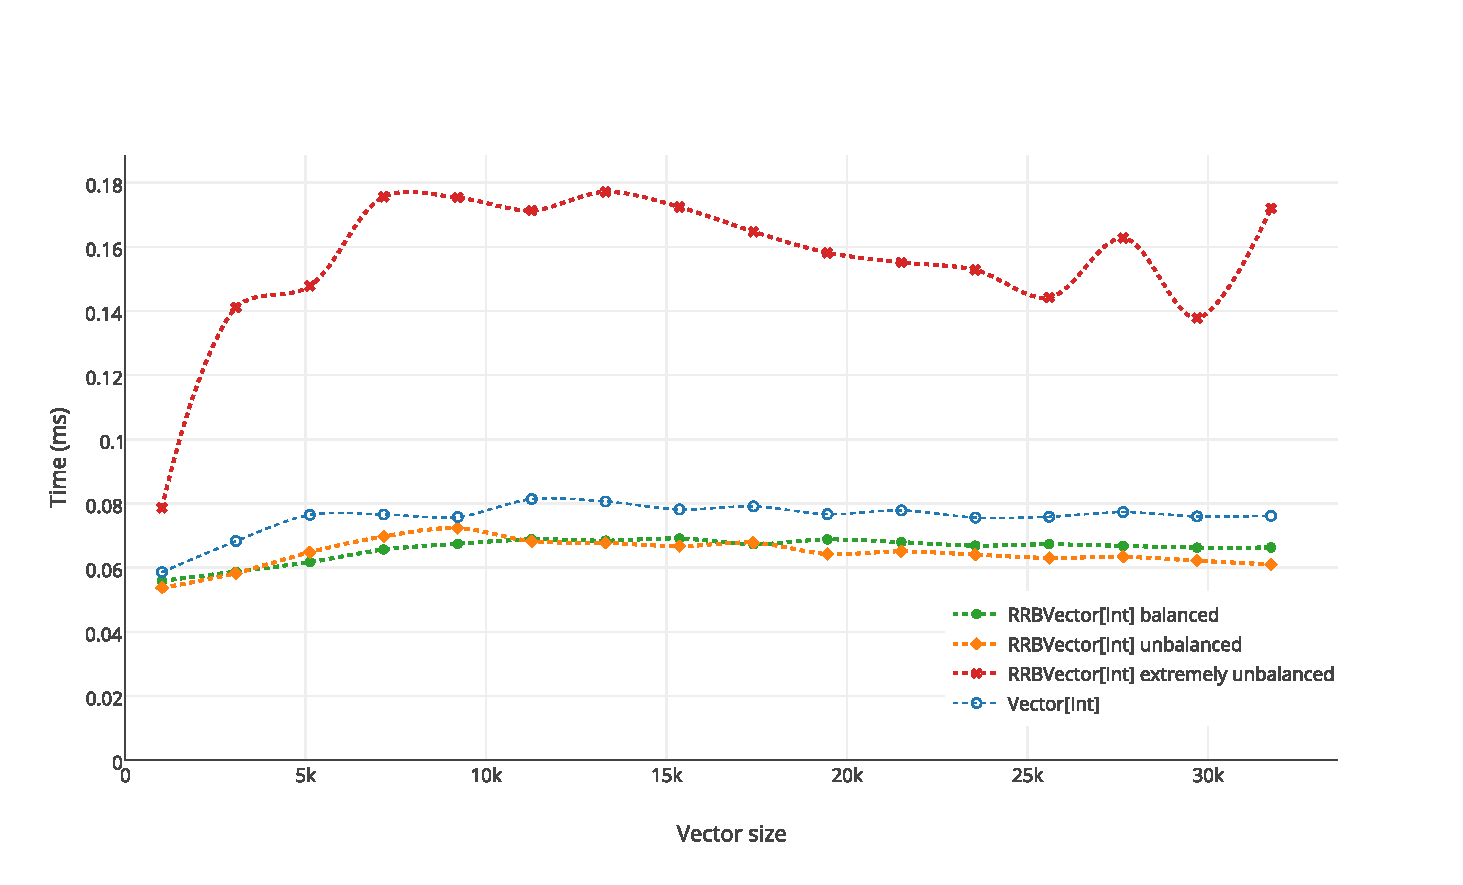
\includegraphics[width=\textwidth]{Benchmarks/Apply_3.pdf}
  \label{ApplyBenchmarks}
  \caption{Time to execute 10k apply operations on sequential indices.}
\end{figure}

\begin{figure}[h!]
  \centering
  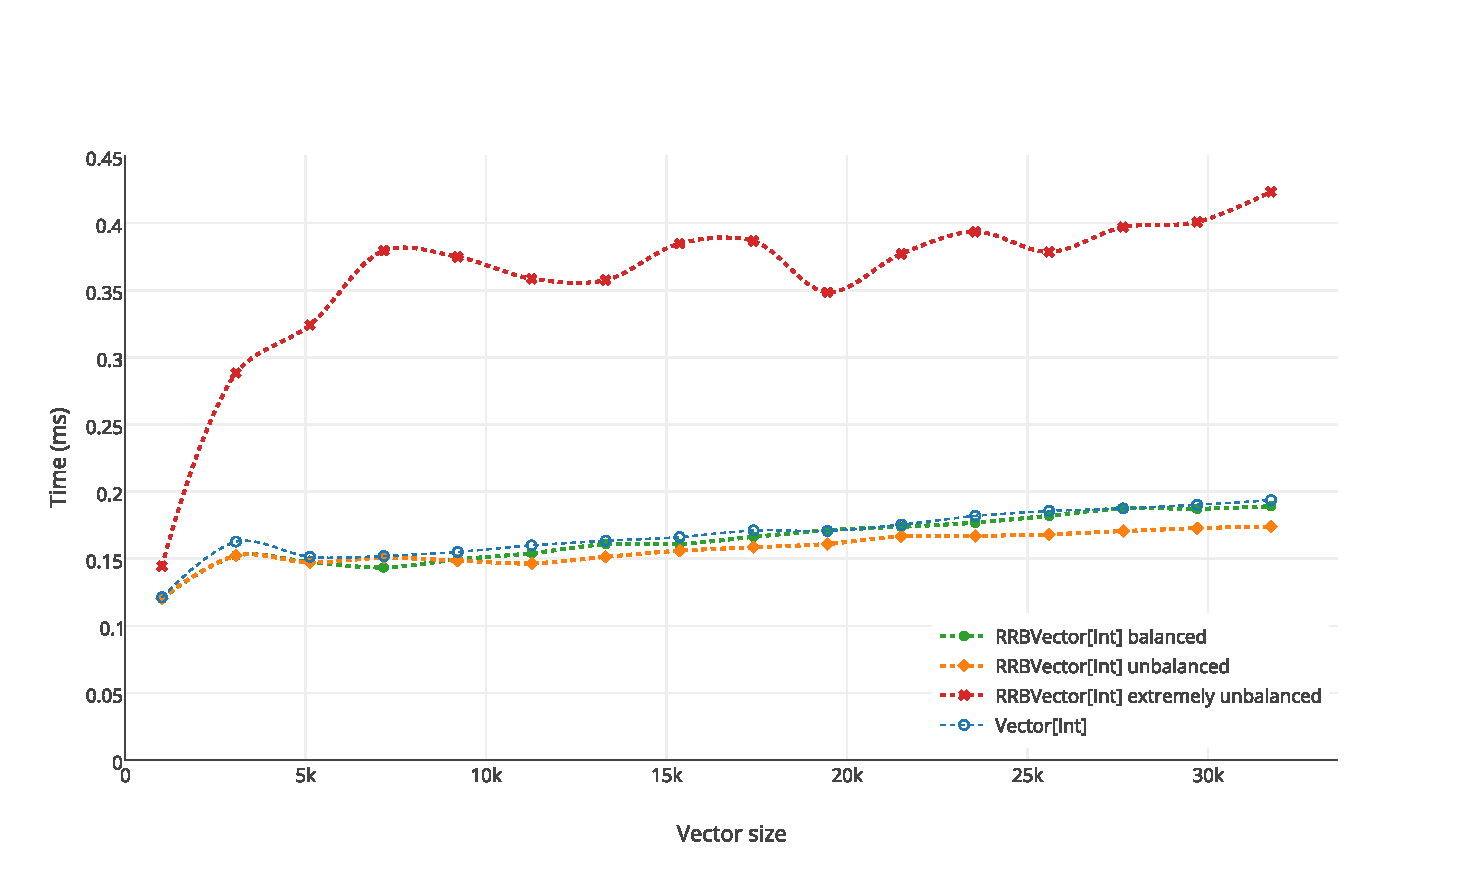
\includegraphics[width=\textwidth]{Benchmarks/Apply_random_3.pdf}
  \label{ApplyRandomBenchmarks}
  \caption{Time to execute 10k apply operations on random indices.}
\end{figure}

\begin{figure}[h!]
  \centering
  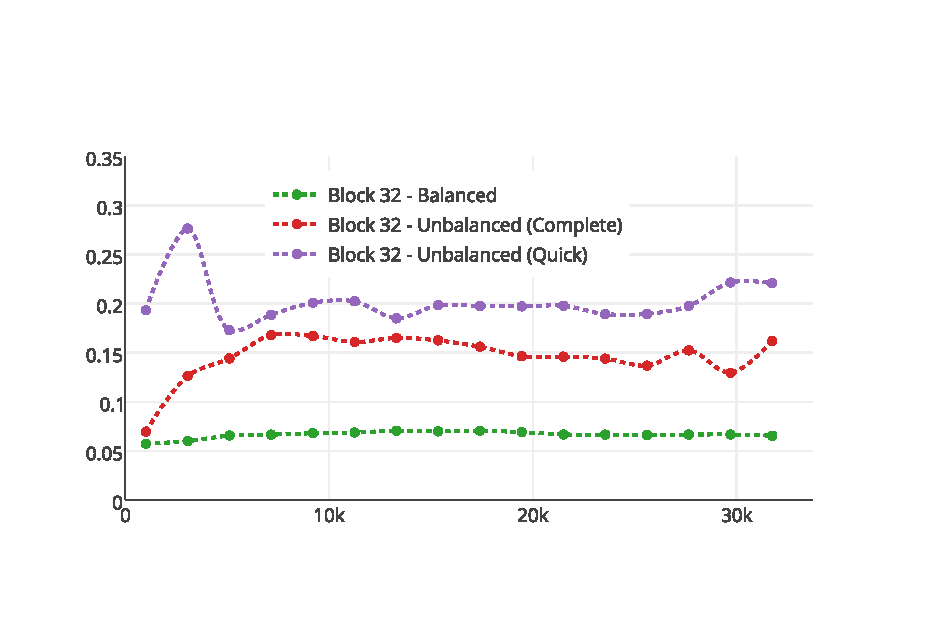
\includegraphics[width=0.49\textwidth]{Benchmarks/Apply_blocks_32.pdf}
  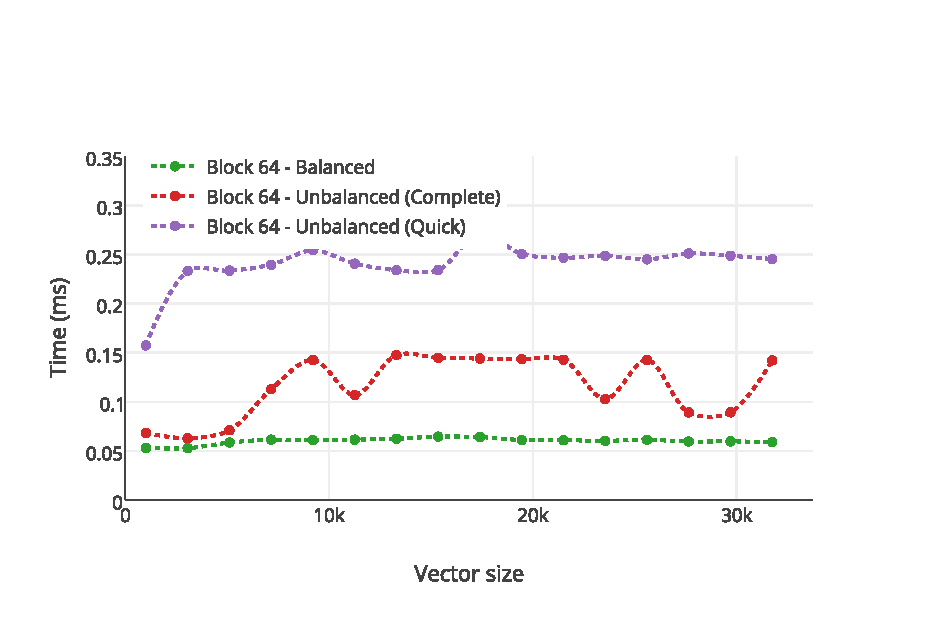
\includegraphics[width=0.49\textwidth]{Benchmarks/Apply_blocks_64.pdf}
  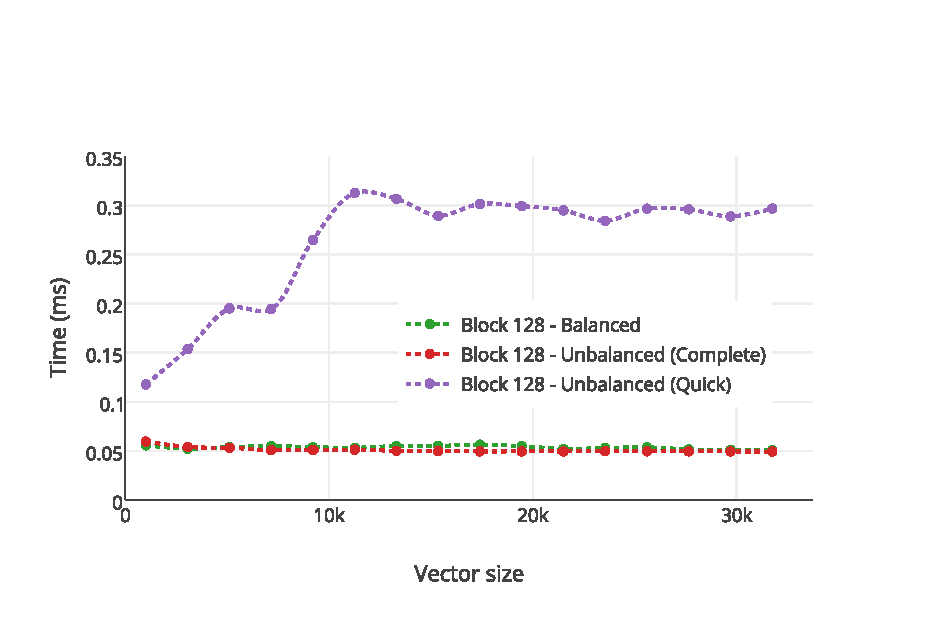
\includegraphics[width=0.49\textwidth]{Benchmarks/Apply_blocks_128.pdf}
  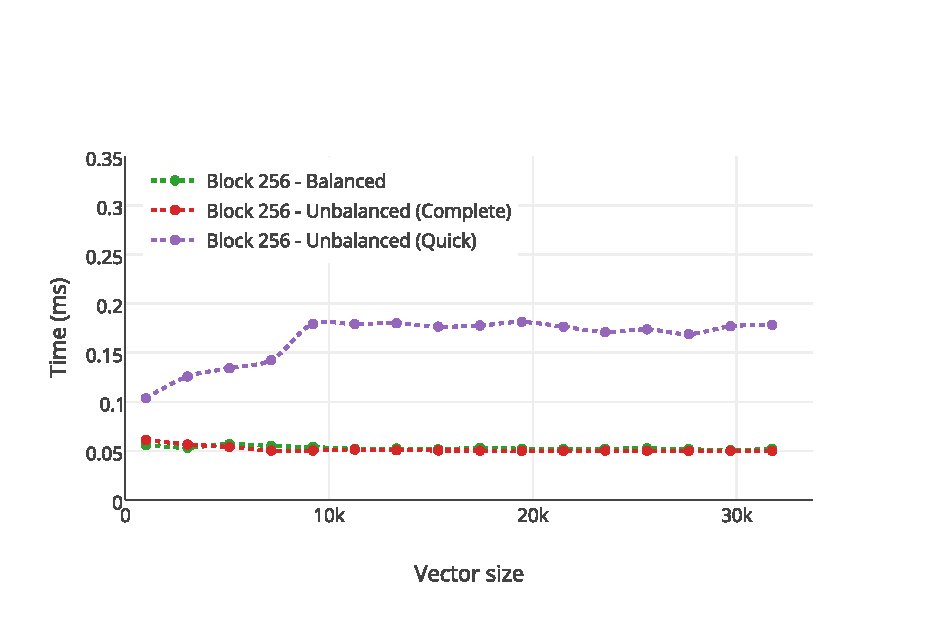
\includegraphics[width=0.49\textwidth]{Benchmarks/Apply_blocks_256.pdf}
  \label{ApplyBlocksBenchmarks}
  \caption{Time to execute 10k apply operations on sequential indices. Comparing performances for different block sizes and different implementation of the concatenation inner branch rebalancing (Complete/Quick).}
\end{figure}

%-----------------------------------
%	SUBSECTION Concatenation
%-----------------------------------
\subsection{Concatenation}
% describe the benchmark function
% compare expectation with results
% explain the upper bound
% explain apparently incoherent results
\color{red} TODO \color{black}

\begin{figure}[h!]
  \centering
  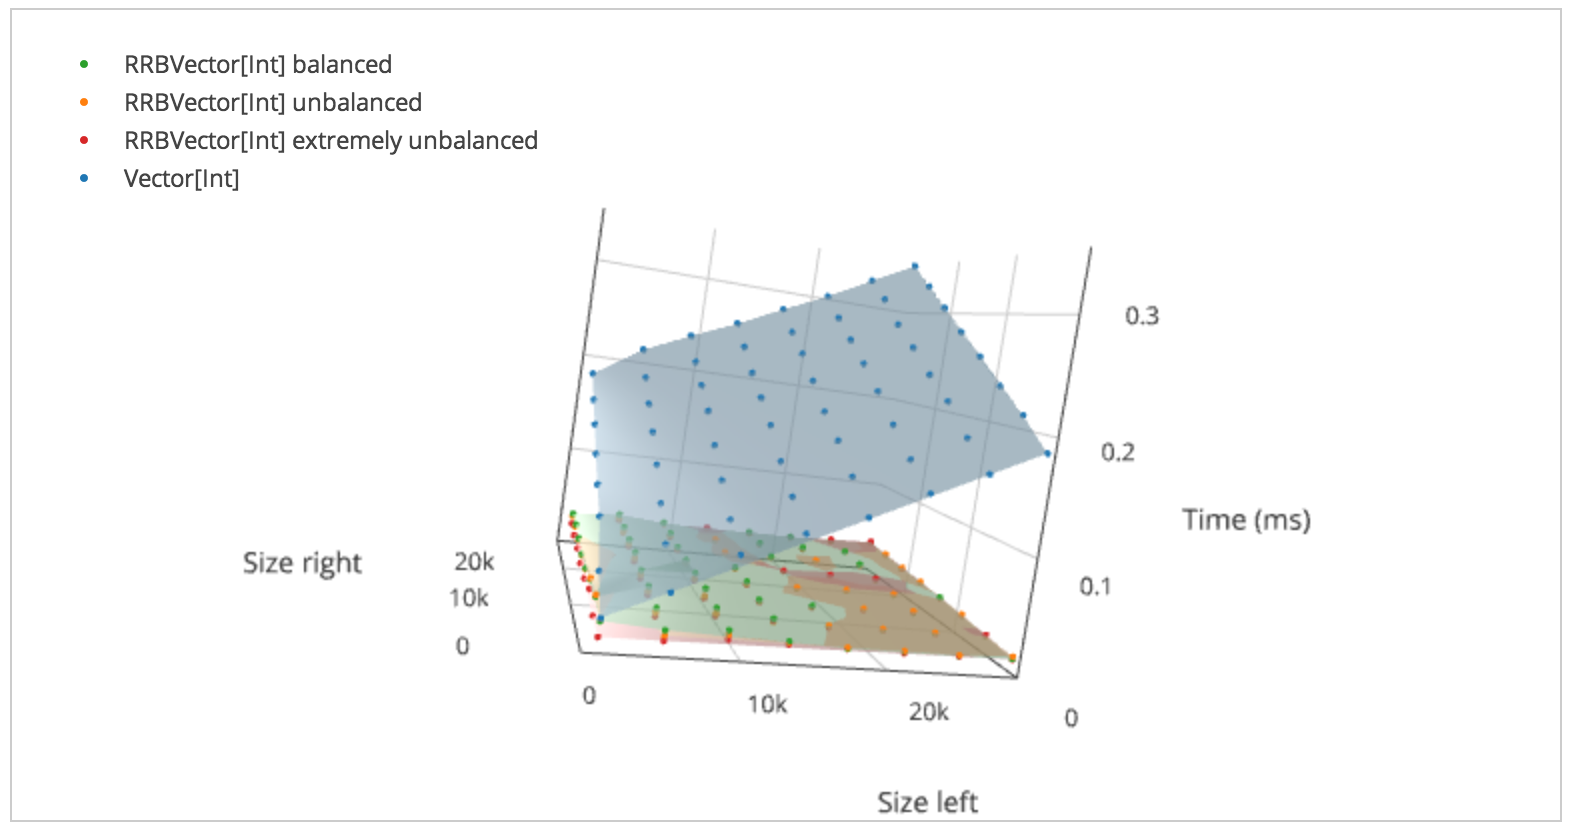
\includegraphics[width=\textwidth]{Benchmarks/Concat.png}
  \label{ConcatBenchmarks}
  \caption{Execution time for a concatenation operation on two vectors. In theory (and in practice) Vector concatenation is $O(left + right)$ and the rrbVector concatenation operation is $O(log_{32}(left + right))$.}
\end{figure}

%-----------------------------------
%	SUBSECTION Append
%-----------------------------------
\subsection{Append}
% describe the benchmark function
% compare expectation with results
% explain the upper bound
% explain apparently incoherent results

\color{red} TODO \color{black}

\begin{figure}[h!]
  \centering
  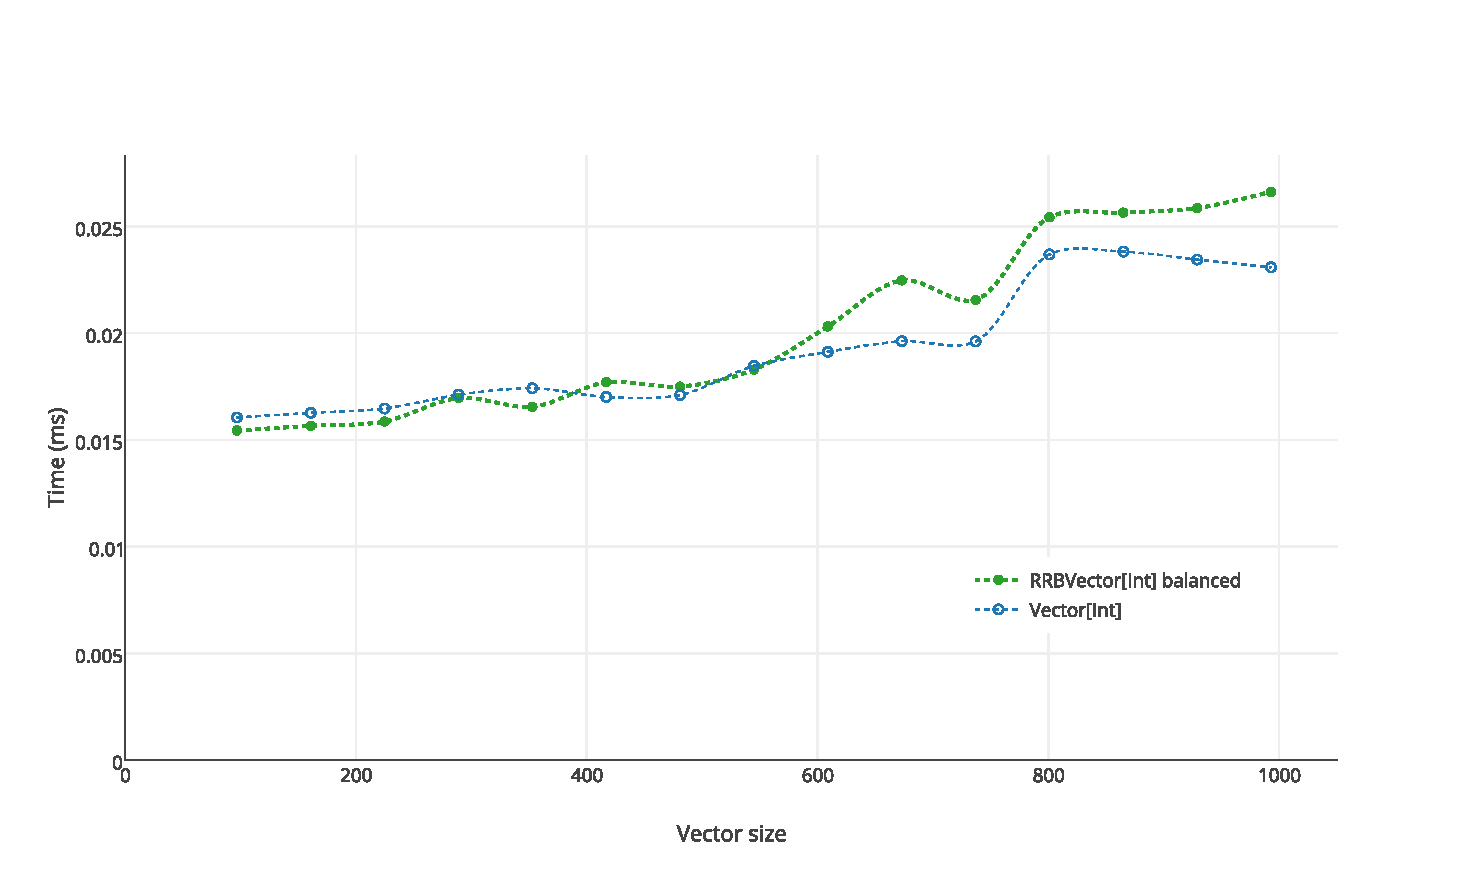
\includegraphics[width=\textwidth]{Benchmarks/Append_2.pdf}
  \label{Append2Benchmarks}
  \caption{Time to execute 256 append operations. This shows the amortized cost of the append operation.}
\end{figure}

\begin{figure}[h!]
  \centering
  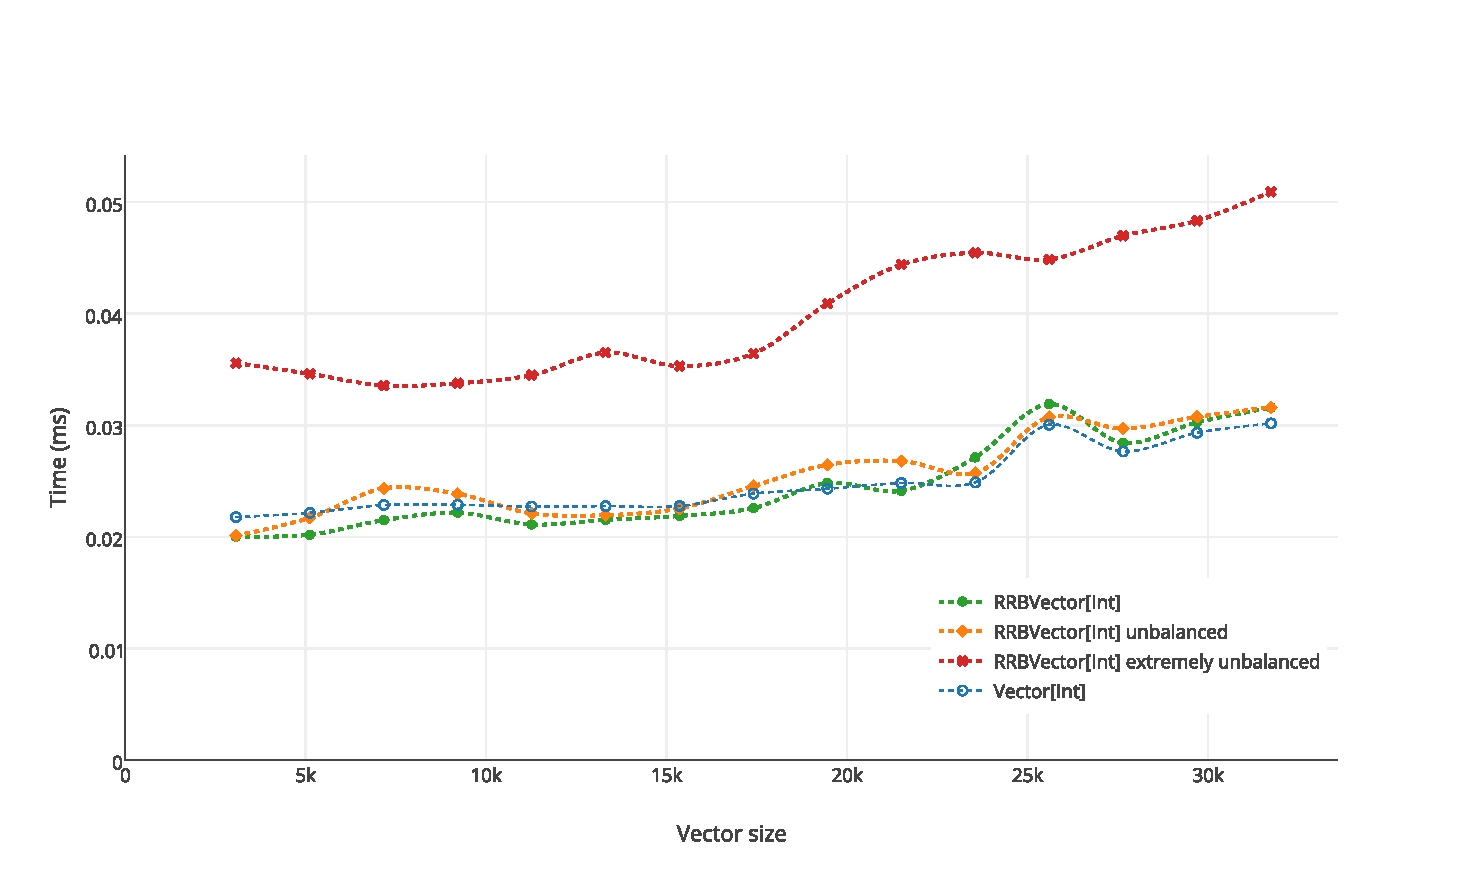
\includegraphics[width=\textwidth]{Benchmarks/Append_3.pdf}
  \label{Append3Benchmarks}
  \caption{Time to execute 256 append operations. This shows the amortized cost of the append operation.}
\end{figure}

\begin{figure}[h!]
  \centering
  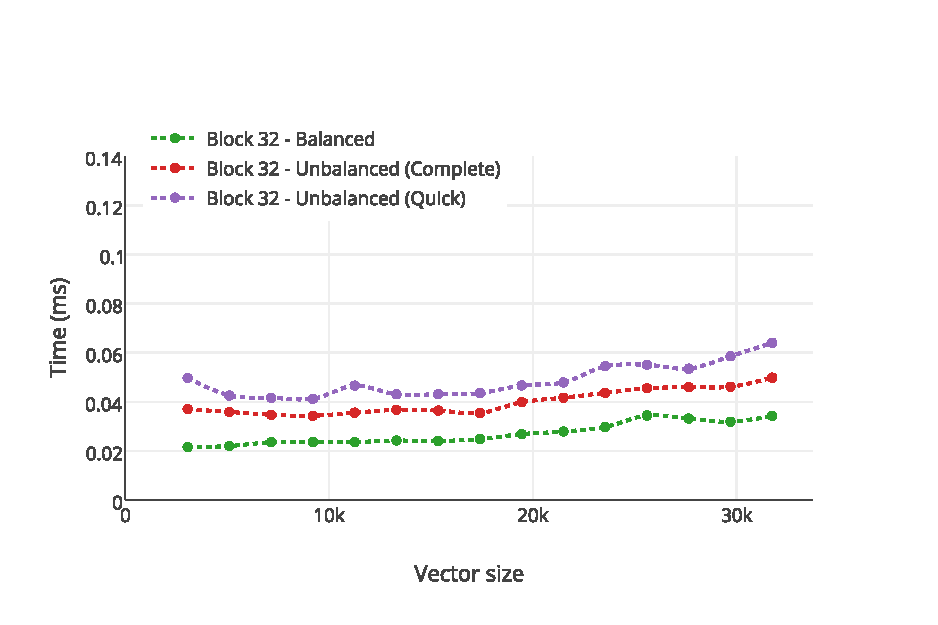
\includegraphics[width=0.49\textwidth]{Benchmarks/Append_blocks_32.pdf}
  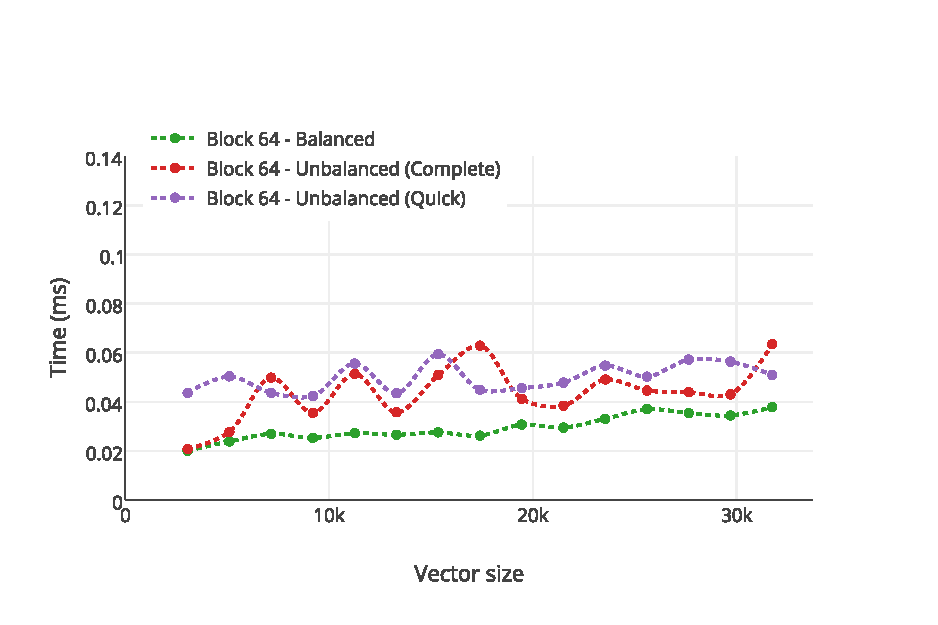
\includegraphics[width=0.49\textwidth]{Benchmarks/Append_blocks_64.pdf}
  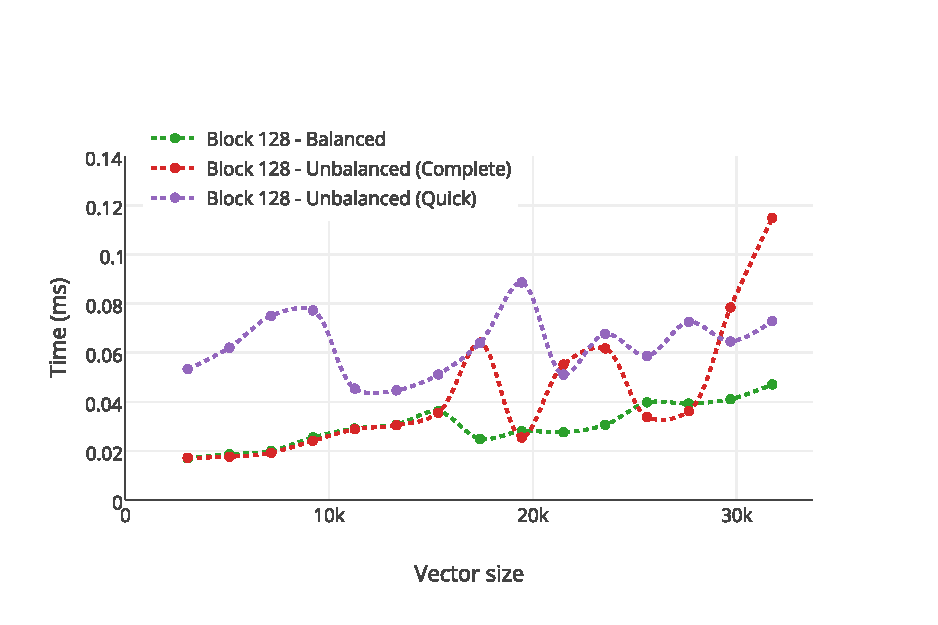
\includegraphics[width=0.49\textwidth]{Benchmarks/Append_blocks_128.pdf}
  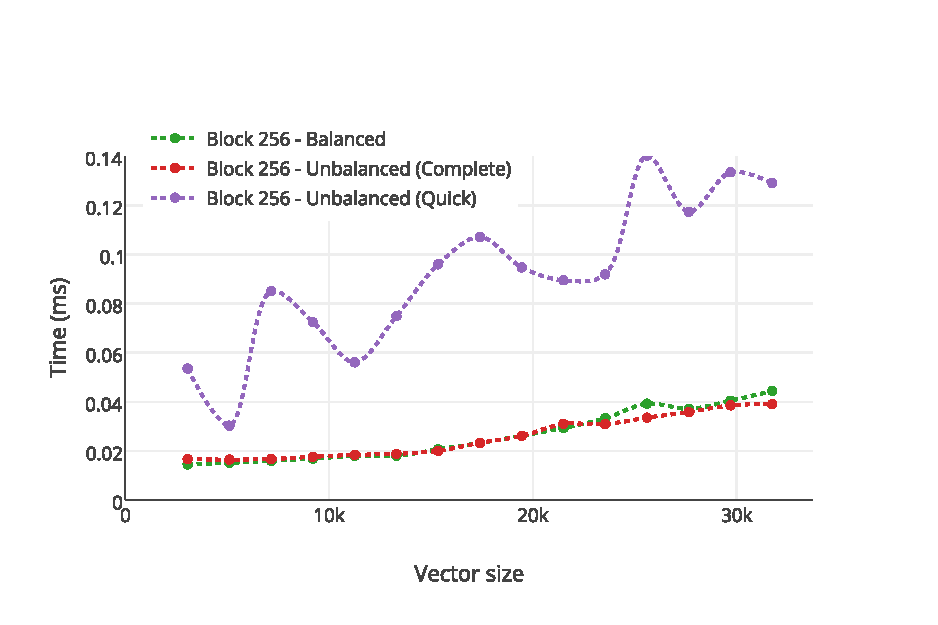
\includegraphics[width=0.49\textwidth]{Benchmarks/Append_blocks_256.pdf}
  \label{IterationBlocksBenchmarks}
  \caption{Time to execute 256 append operations. This shows the amortized cost of the append operation. Comparing performances for different block sizes and different implementation of the concatenation inner branch rebalancing (Complete/Quick).}
\end{figure}

%-----------------------------------
%	SUBSECTION Prepend
%-----------------------------------
\subsection{Prepend}
% describe the benchmark function
% compare expectation with results
% explain the upper bound
% explain apparently incoherent results
\color{red} TODO \color{black}

\begin{figure}[h!]
  \centering
  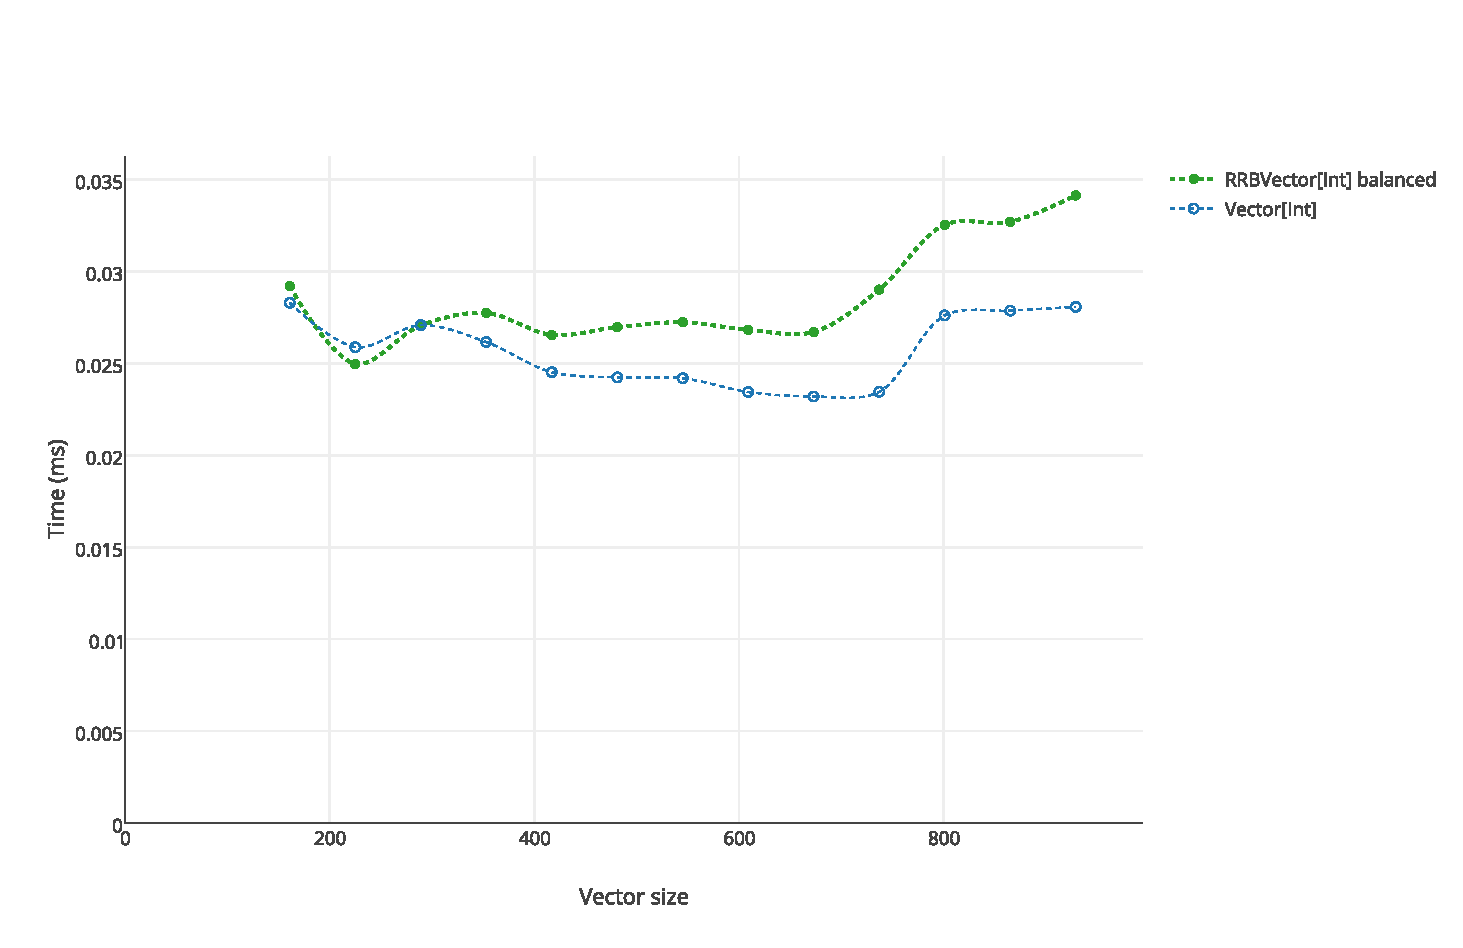
\includegraphics[width=\textwidth]{Benchmarks/Prepend_2.pdf}
  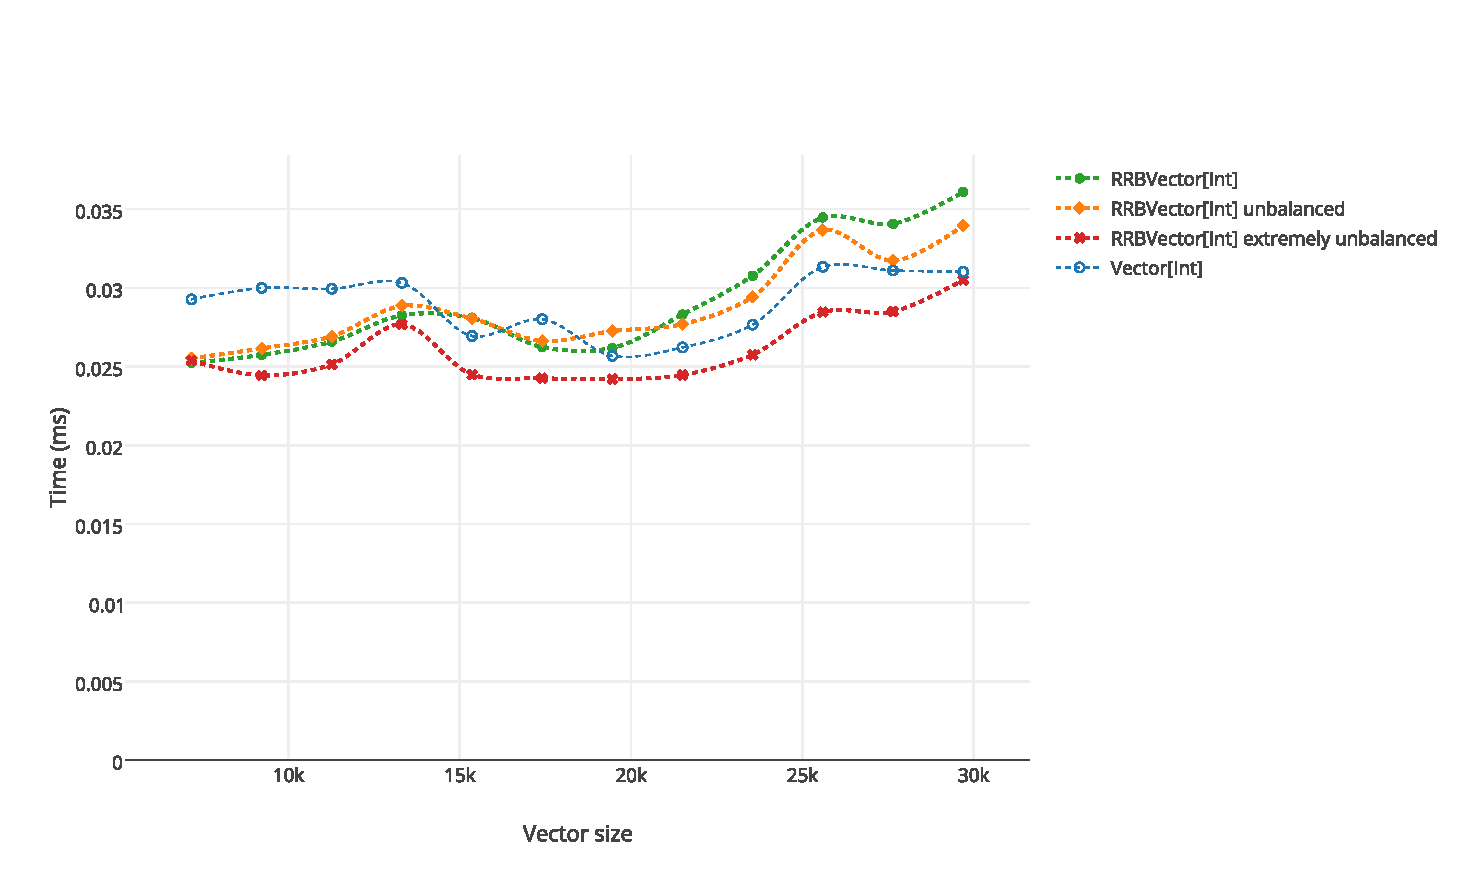
\includegraphics[width=\textwidth]{Benchmarks/Prepend_3.pdf}
  \label{PrependBenchmarks}
  \caption{Time to execute 256 prepend operations. This shows the amortized cost of the prepend operation.}
\end{figure}

\begin{figure}[h!]
  \centering
  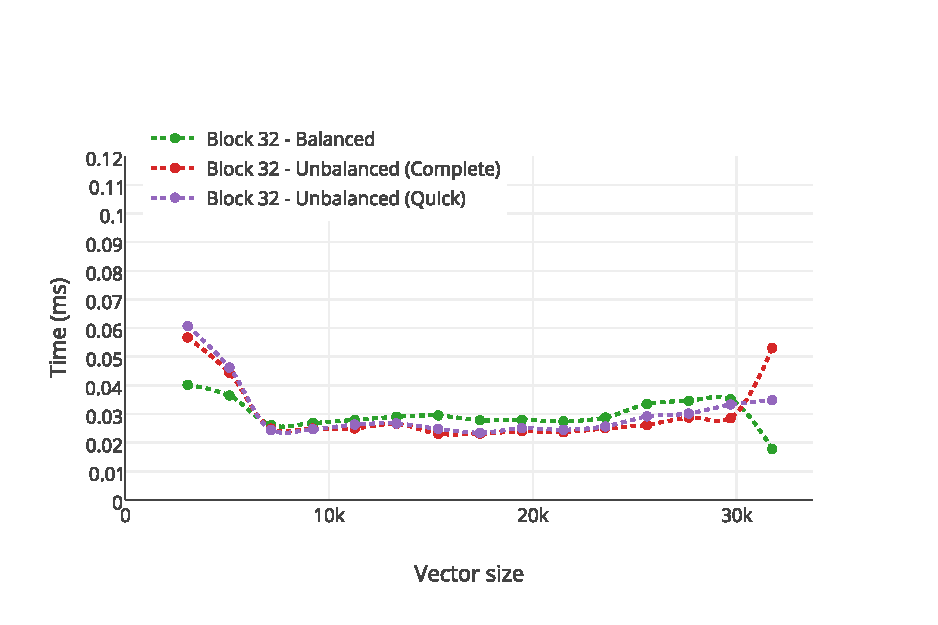
\includegraphics[width=0.49\textwidth]{Benchmarks/Prepend_blocks_32.pdf}
  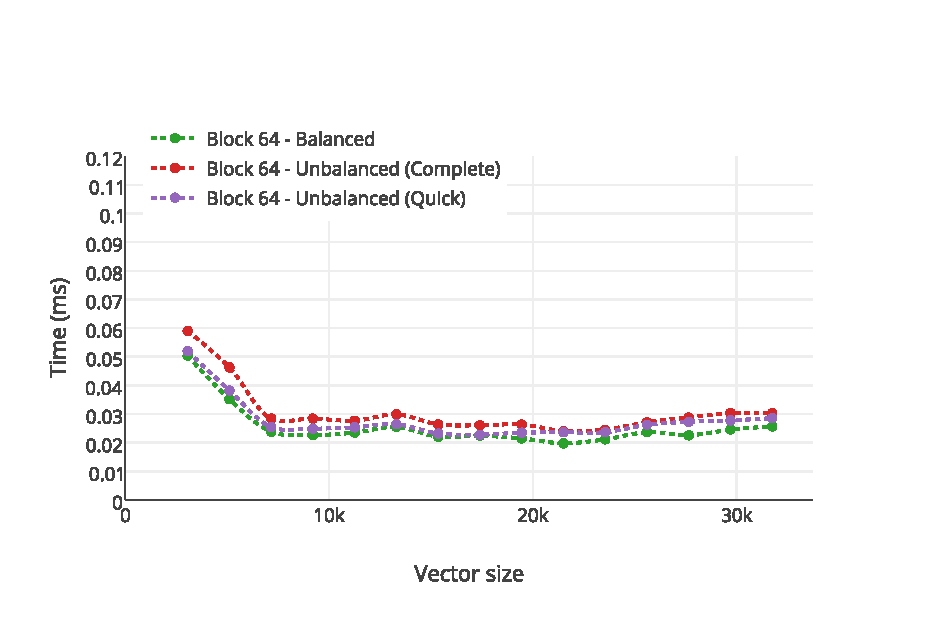
\includegraphics[width=0.49\textwidth]{Benchmarks/Prepend_blocks_64.pdf}
  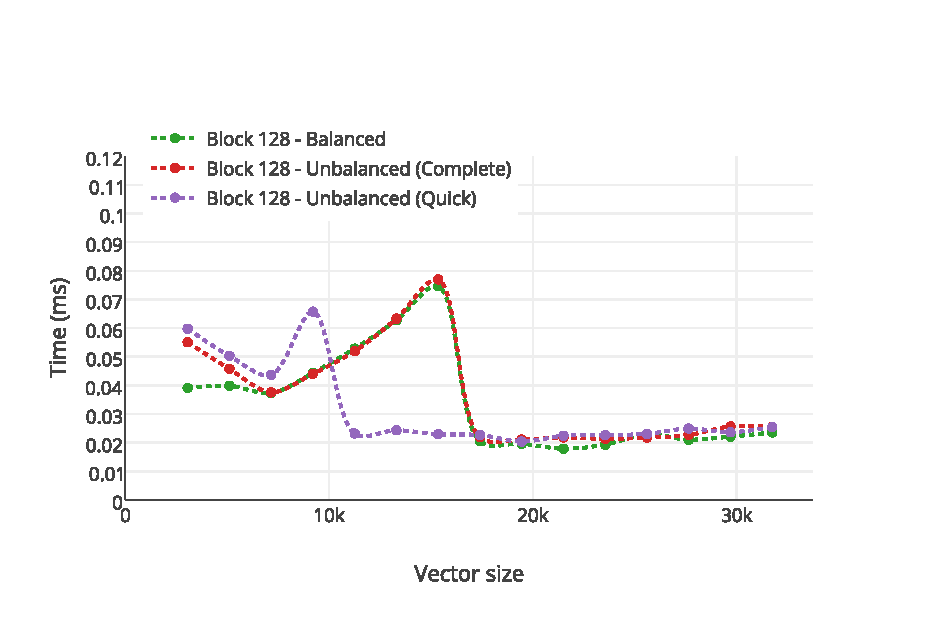
\includegraphics[width=0.49\textwidth]{Benchmarks/Prepend_blocks_128.pdf}
  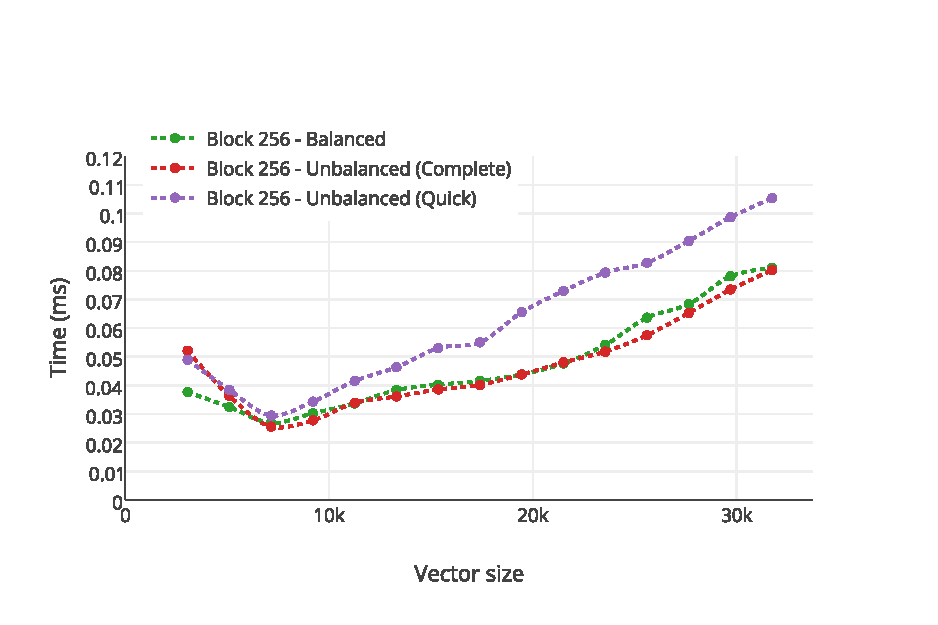
\includegraphics[width=0.49\textwidth]{Benchmarks/Prepend_blocks_256.pdf}
  \label{PrependBenchmarks}
  \caption{Time to execute 256 prepend operations. This shows the amortized cost of the append operation. Comparing performances for different block sizes and different implementation of the concatenation inner branch rebalancing (Complete/Quick).}
\end{figure}


%-----------------------------------
%	SUBSECTION Splits
%-----------------------------------
\subsection{Splits}
% describe the benchmark function
% compare expectation with results
% explain the upper bound
% explain apparently incoherent results
\color{red} TODO \color{black}

\begin{figure}[h!]
  \centering
  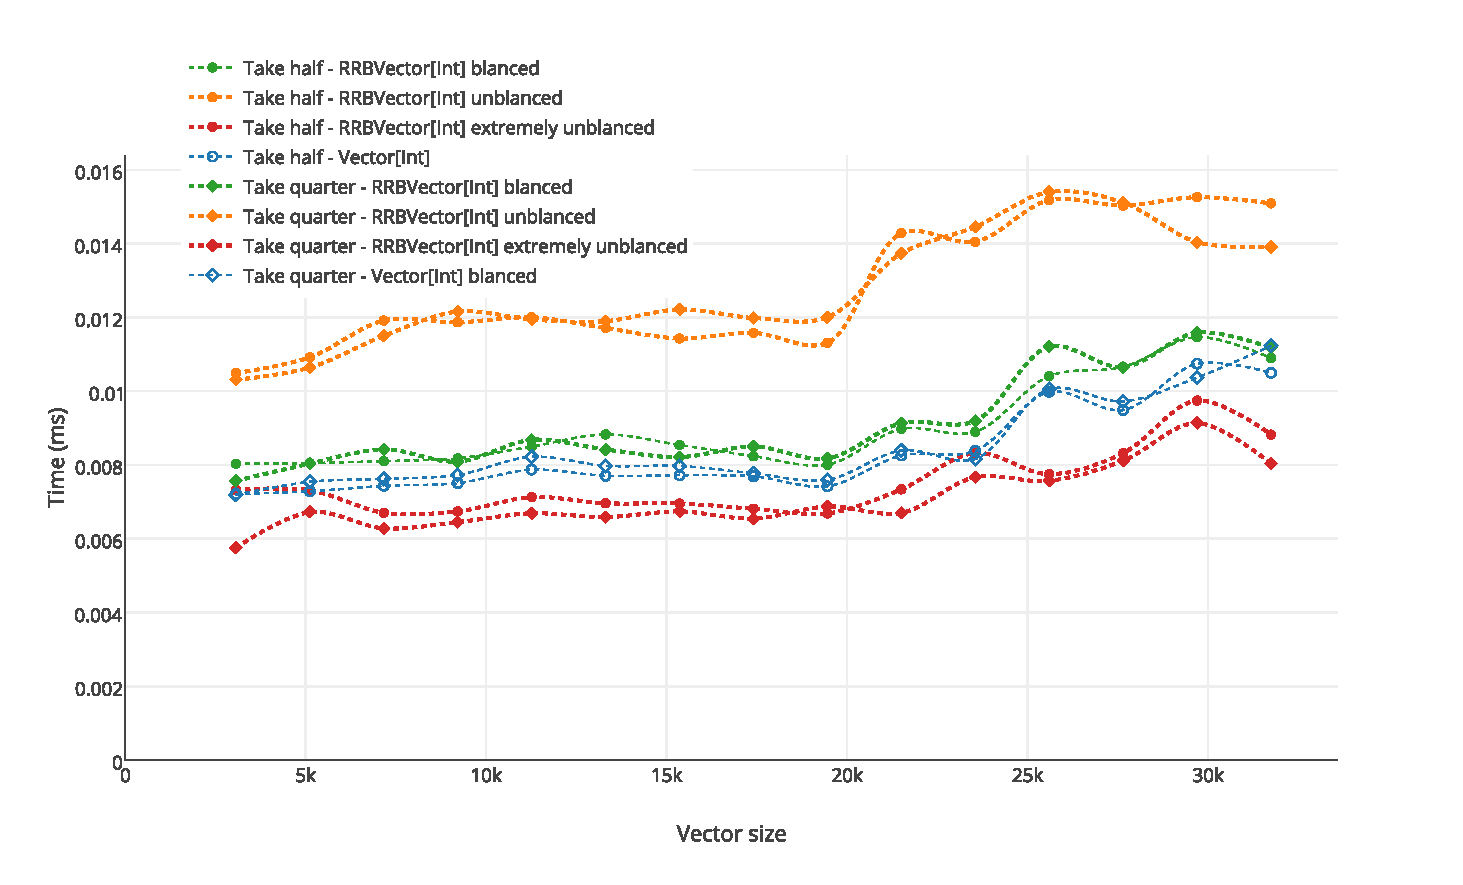
\includegraphics[width=\textwidth]{Benchmarks/Split_take_3.pdf}
  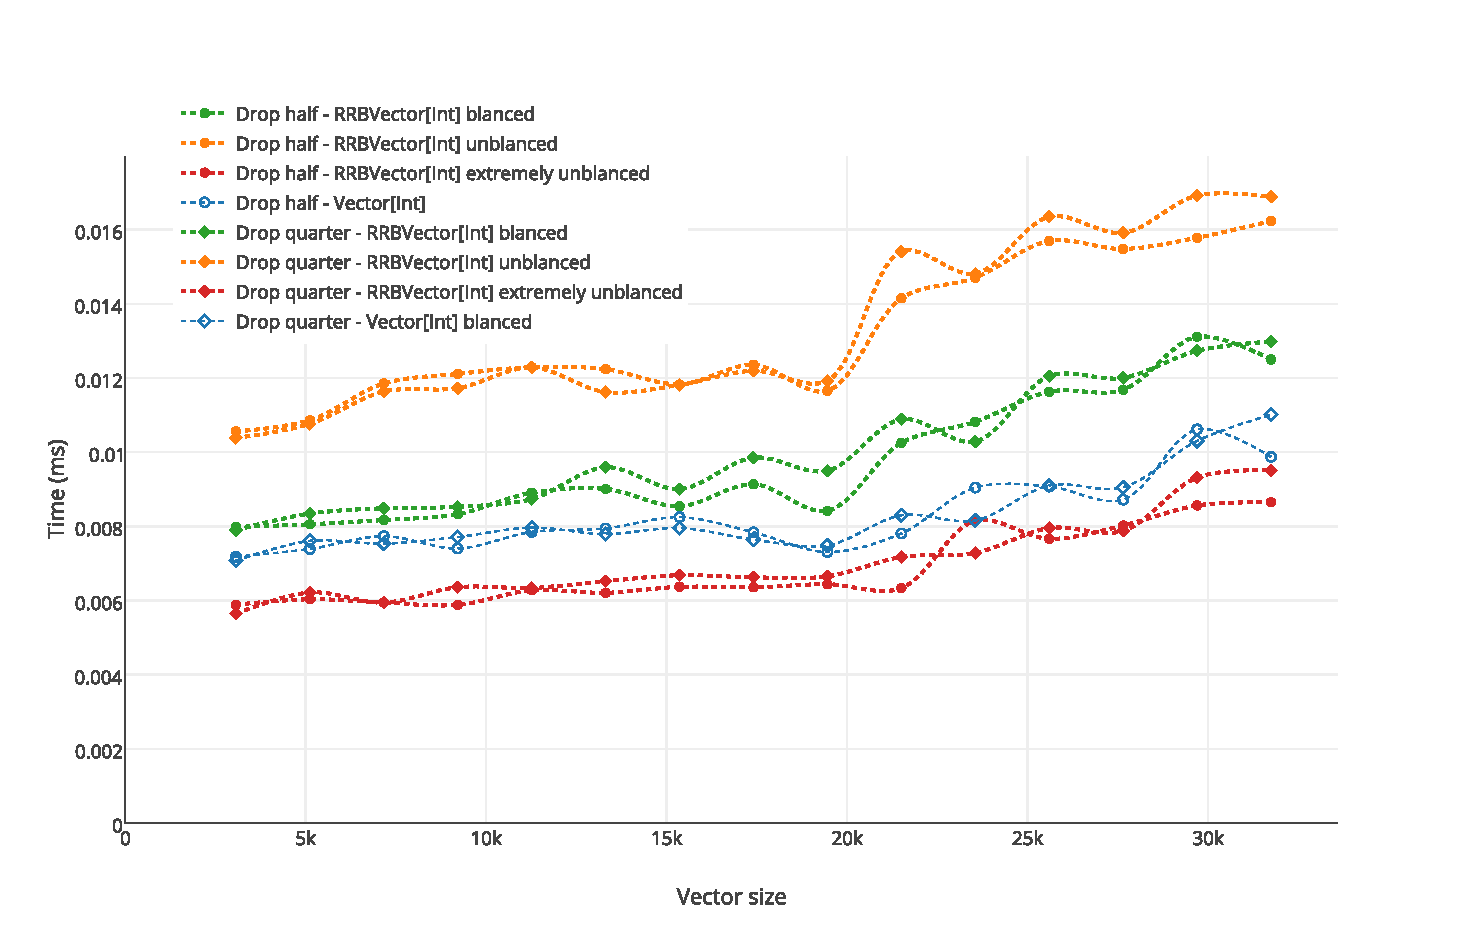
\includegraphics[width=\textwidth]{Benchmarks/Split_drop_3.pdf}
  \label{SplitsBenchmarks}
  \caption{Execution time of take and drop.}
\end{figure}


%-----------------------------------
%	SUBSECTION Iterator
%-----------------------------------
\subsection{Iterator}
% describe the benchmark function
% compare expectation with results
% explain the upper bound
% explain apparently incoherent results: iteration of sightly unbalanced vector is faster
\color{red} TODO \color{black}

\begin{figure}[h!]
  \centering
  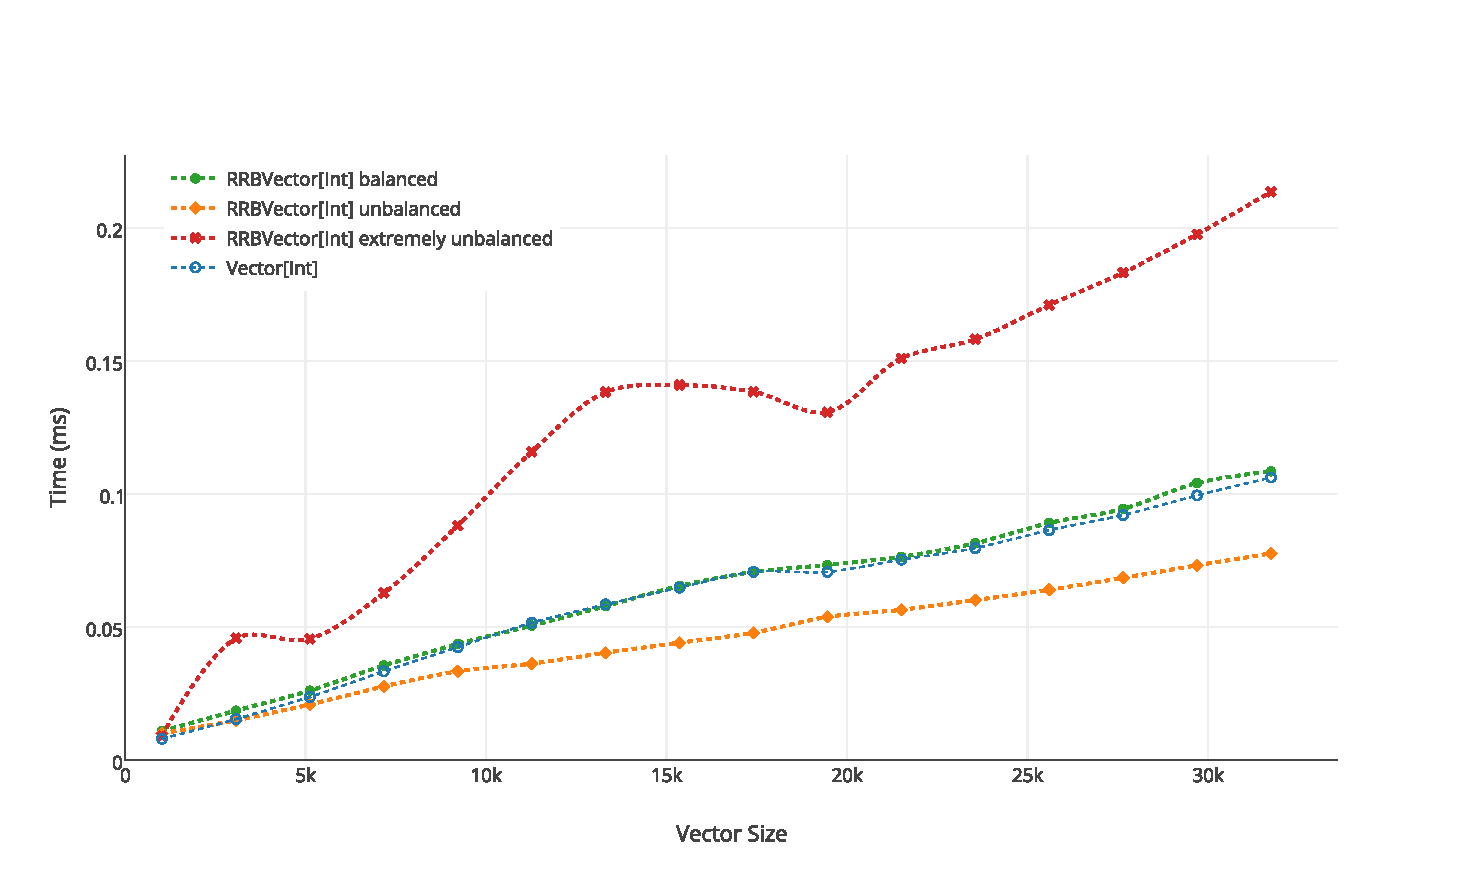
\includegraphics[width=\textwidth]{Benchmarks/Iteration_3.pdf}
  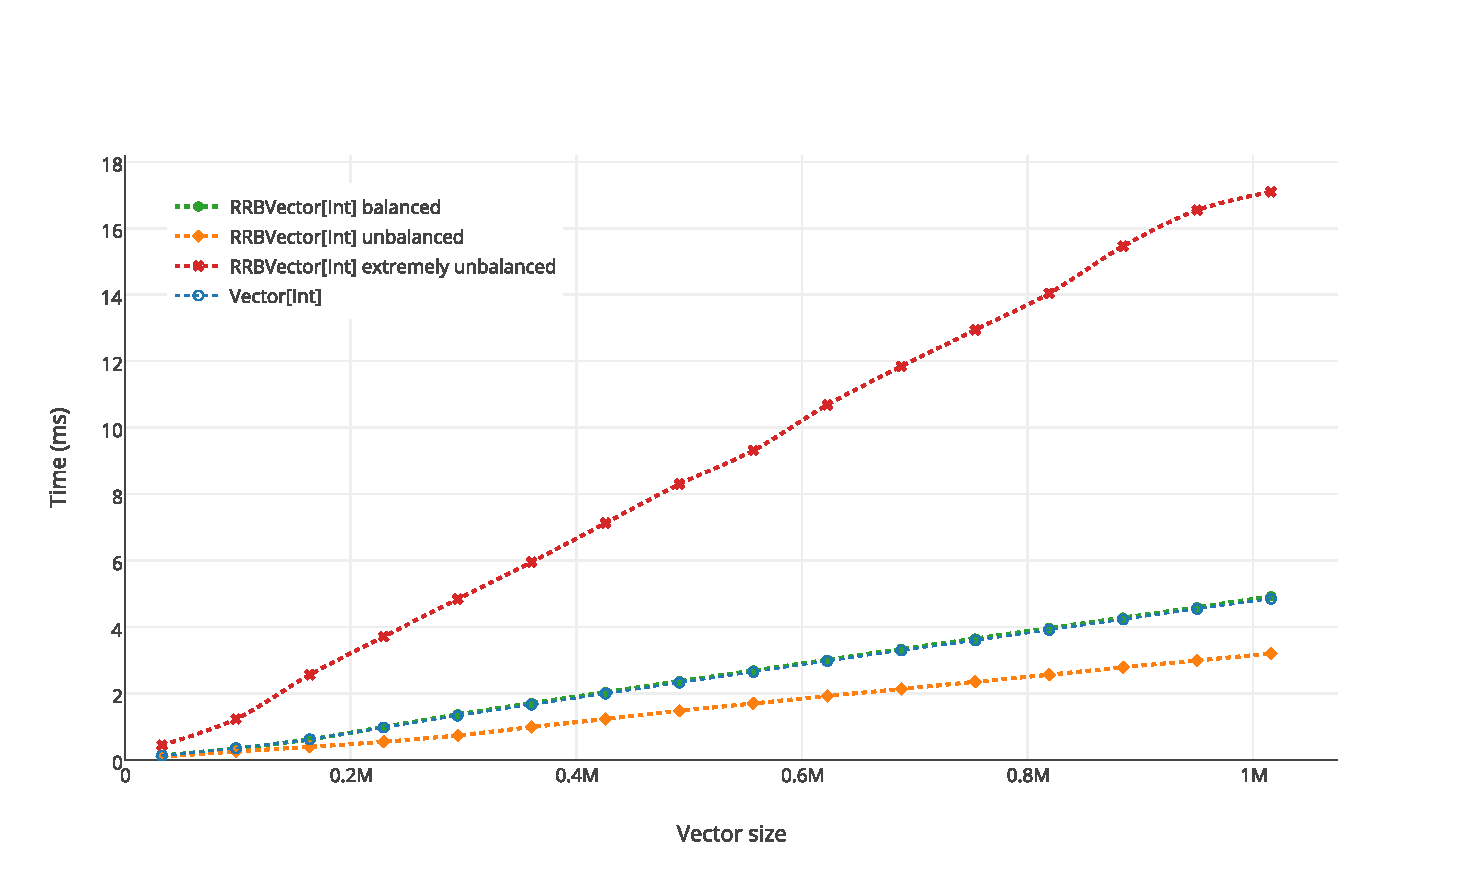
\includegraphics[width=\textwidth]{Benchmarks/Iteration_4.pdf}
  \label{IterationBenchmarks}
  \caption{Excecution time to iterate through all the elements of the vector.}
\end{figure}

\begin{figure}[h!]
  \centering
  \label{IterationBlocksBenchmarks}
  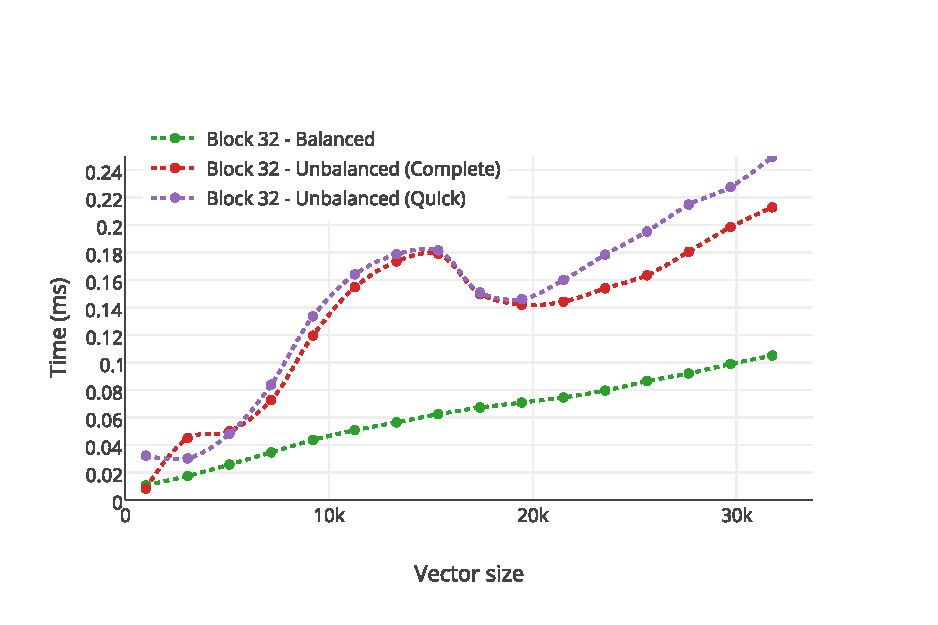
\includegraphics[width=0.49\textwidth]{Benchmarks/Iteration_blocks_32.pdf}
  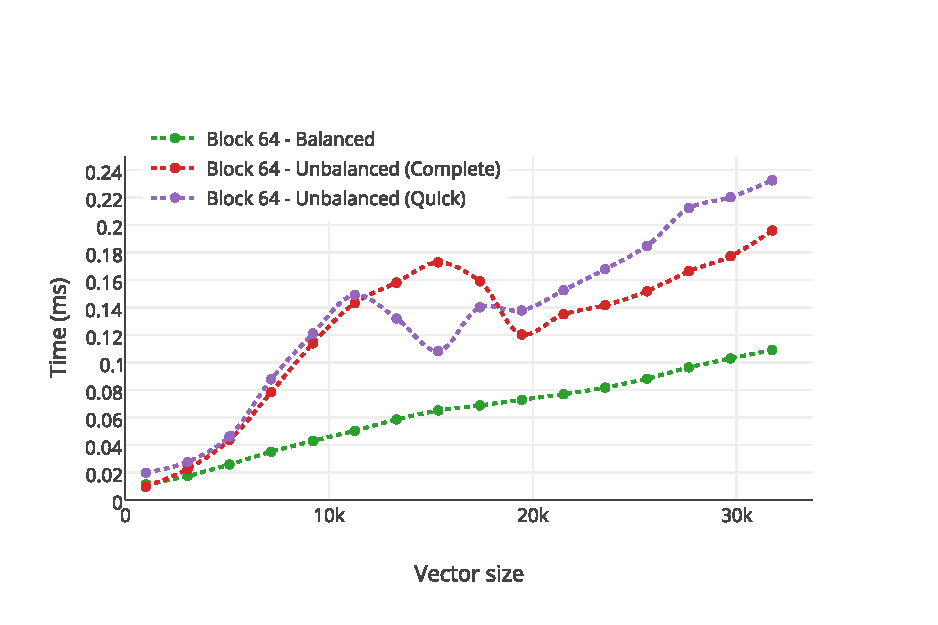
\includegraphics[width=0.49\textwidth]{Benchmarks/Iteration_blocks_64.pdf}
  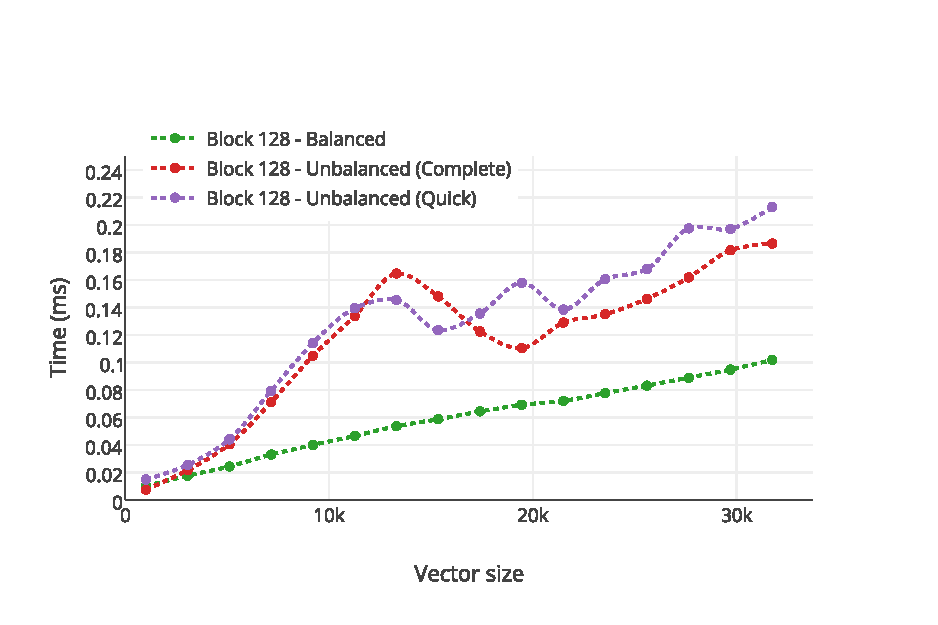
\includegraphics[width=0.49\textwidth]{Benchmarks/Iteration_blocks_128.pdf}
  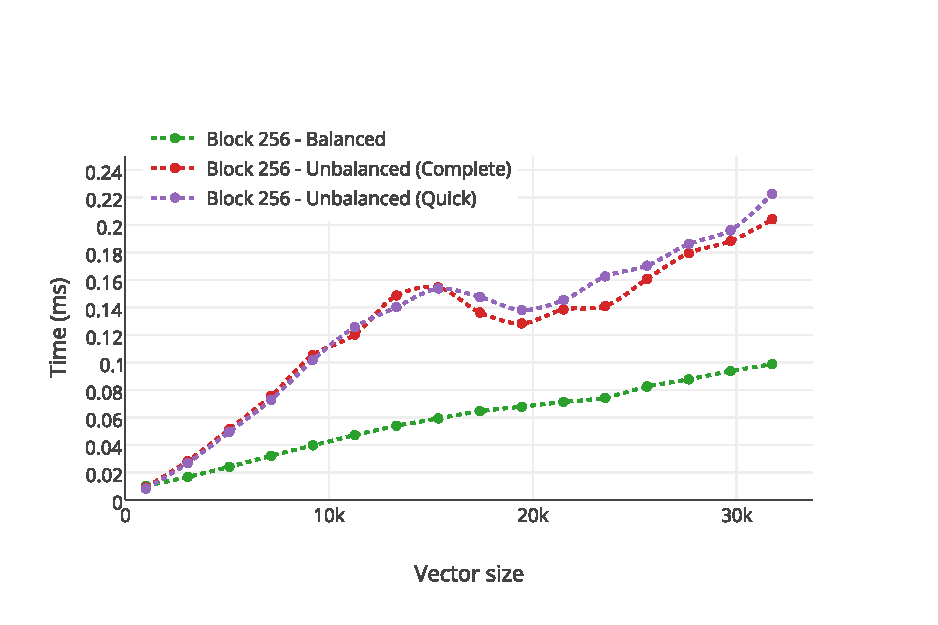
\includegraphics[width=0.49\textwidth]{Benchmarks/Iteration_blocks_256.pdf}
  \caption{Excecution time to iterate through all the elements of the vector. Comparing performances for different block sizes and different implementation of the concatenation inner branch rebalancing (Complete/Quick).}
\end{figure}

%-----------------------------------
%	SUBSECTION Builder
%-----------------------------------
\subsection{Builder}
% describe the benchmark function
% compare expectation with results
% explain the upper bound
% explain apparently incoherent results
\color{red} TODO \color{black}

\begin{figure}[h!]
  \centering
  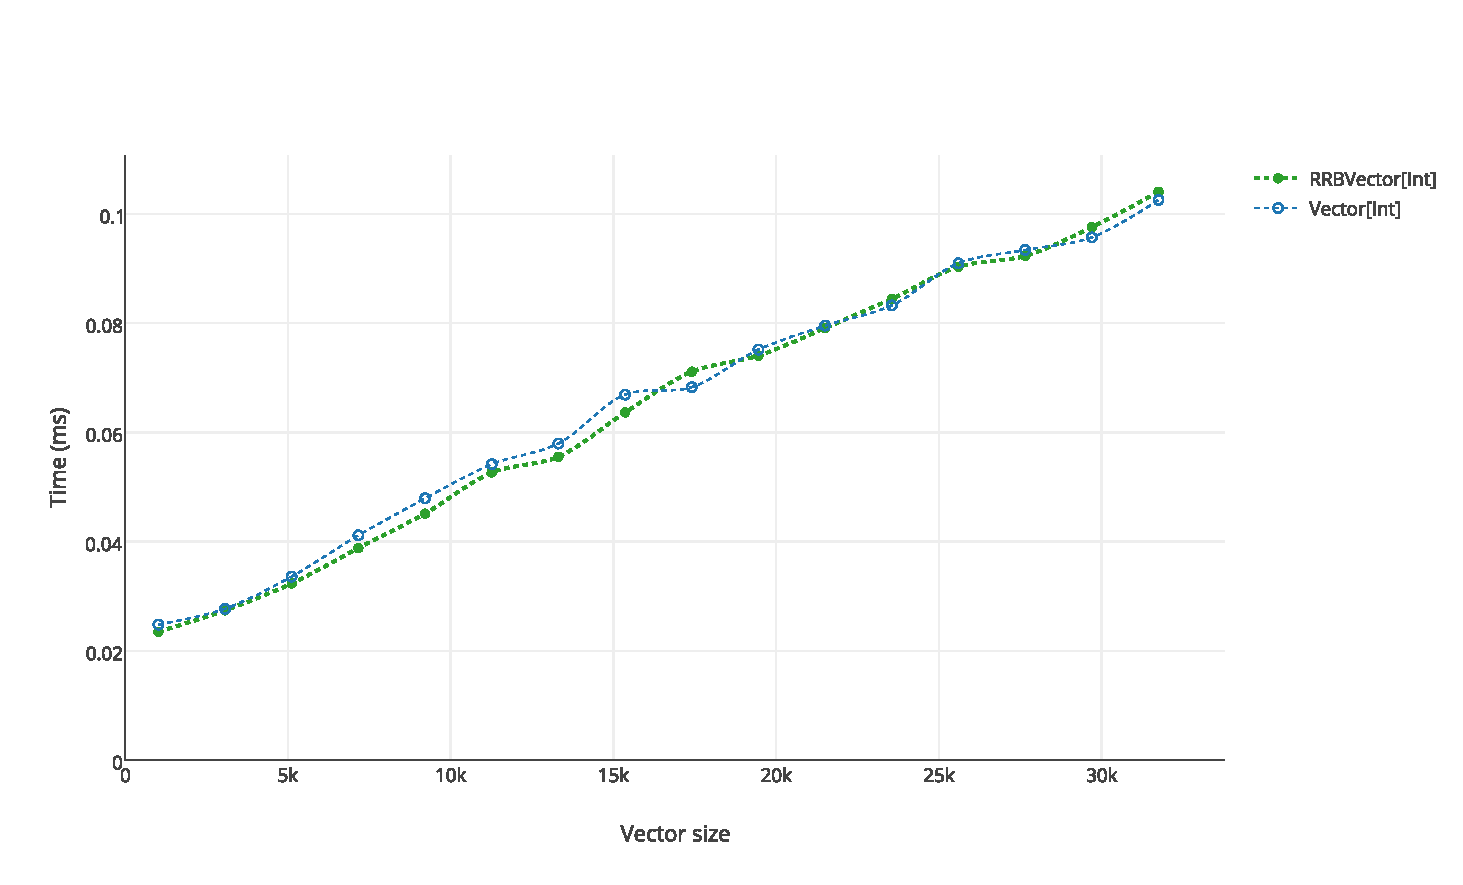
\includegraphics[width=\textwidth]{Benchmarks/Builder_3.pdf}
  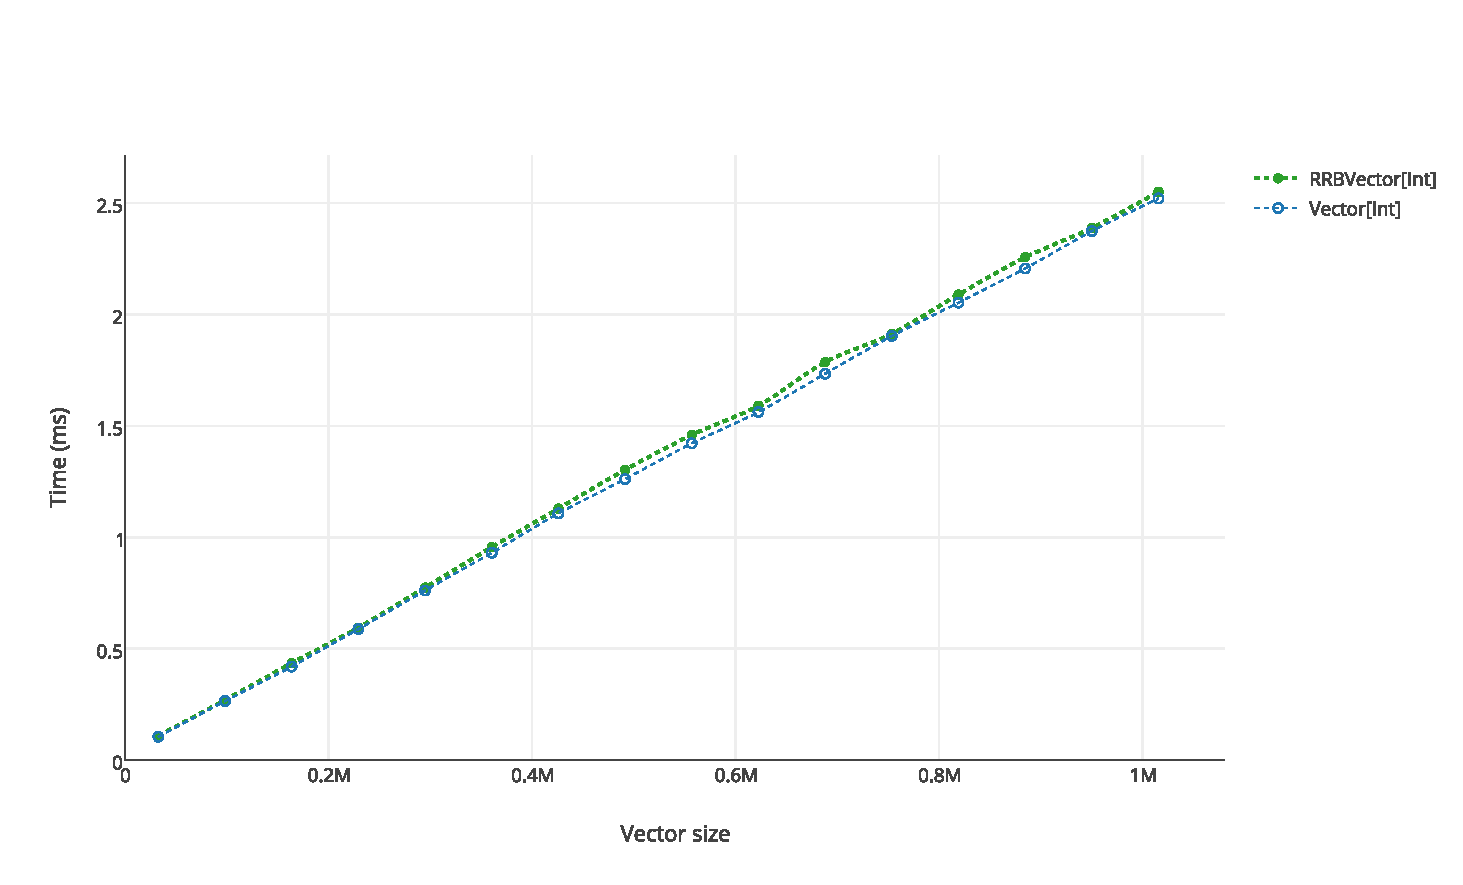
\includegraphics[width=\textwidth]{Benchmarks/Builder_4.pdf}
  \label{BuilderBenchmarks}
  \caption{Execution time to build a vector of a given size.}
\end{figure}

\begin{figure}[h!]
  \centering
  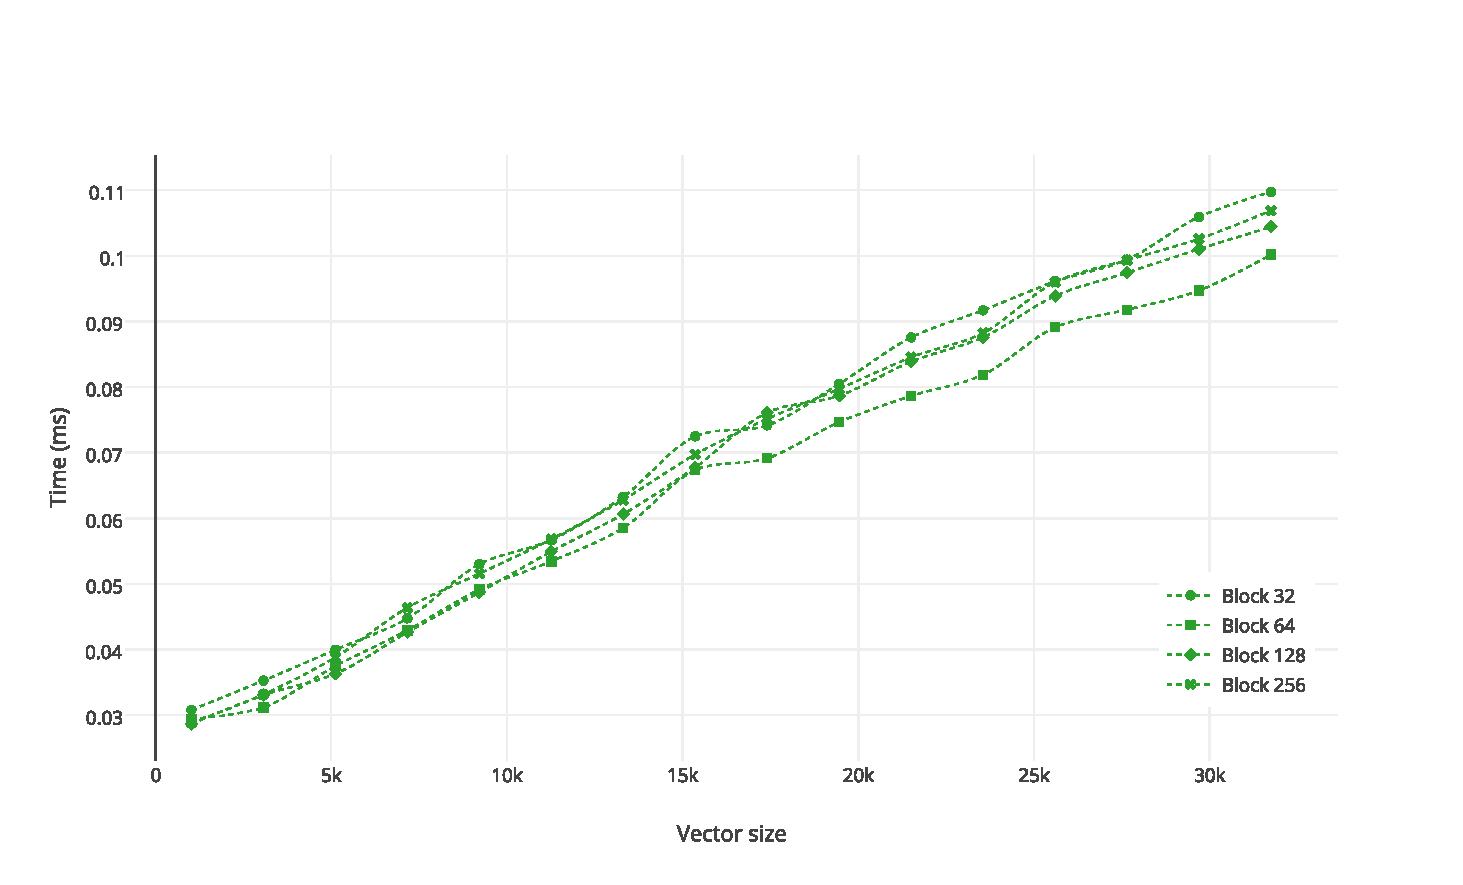
\includegraphics[width=\textwidth]{Benchmarks/Builder_blocks.pdf}
  \label{BuilderBlocksBenchmarks}
  \caption{Execution time to build a vector of a given size. Comparing performances for different block sizes.}
\end{figure}

%-----------------------------------
%	SUBSECTION Parallel split-combine
%-----------------------------------
\subsection{Parallel split-combine}
% describe the benchmark function
% compare expectation with results
% explain the upper bound
% explain apparently incoherent results
\color{red} TODO \color{black}

\begin{figure}[h!]
  \centering
  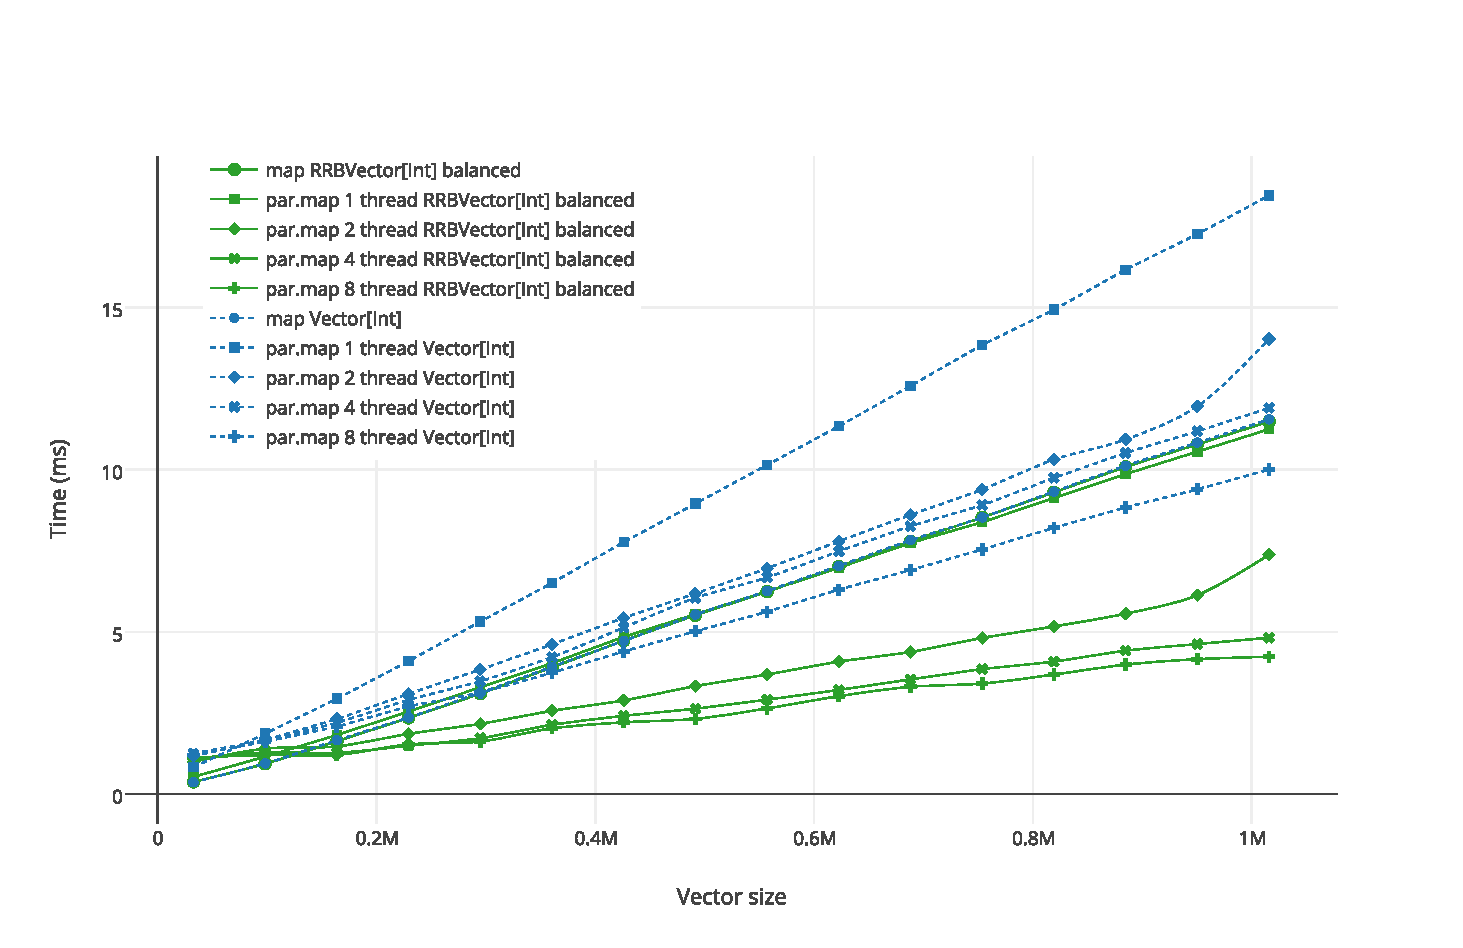
\includegraphics[width=\textwidth]{Benchmarks/Parmap_balanced.pdf}
  \label{ParallelBenchmarks}
  \caption{Benchmark on map and parallel map using the function (\textsc{x=>x}) to show the difference time used in the framework. This time represents the time spent in the splitters and combiners of the parallel collection (iterator and builder for the sequential version).}
\end{figure}

\begin{figure}[h!]
  \centering
  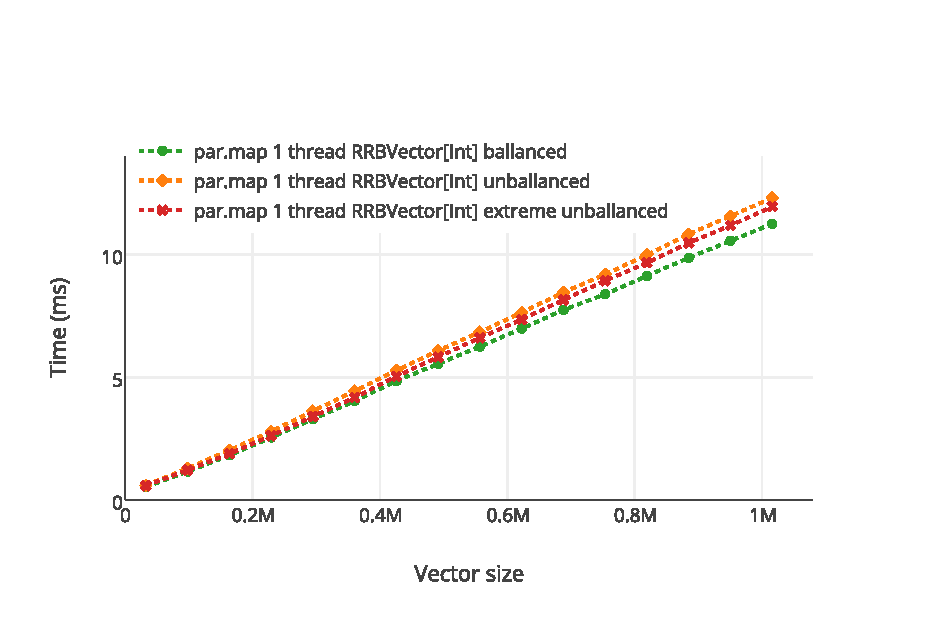
\includegraphics[width=0.49\textwidth]{Benchmarks/parmap_unbalanced_1.pdf}
  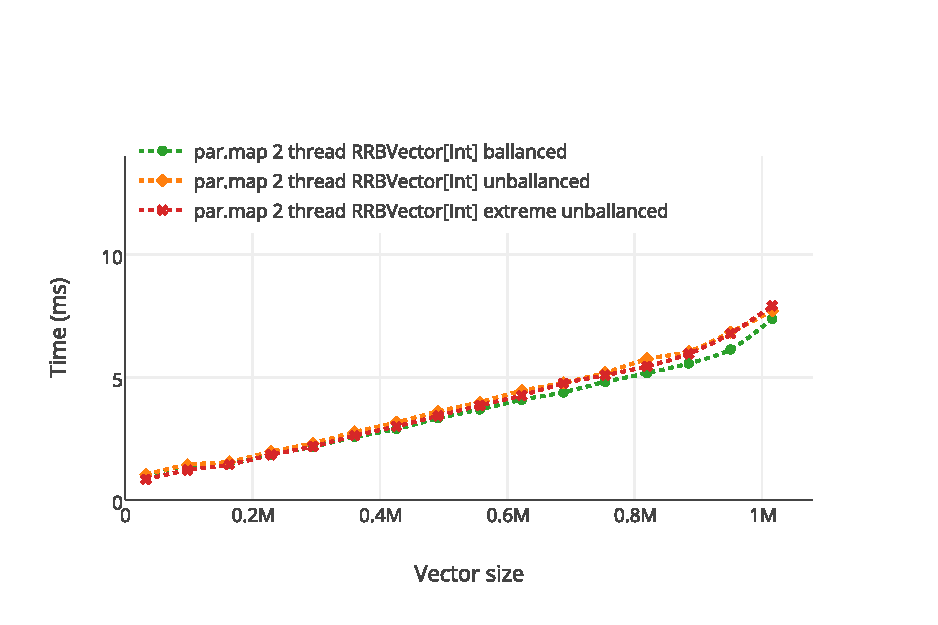
\includegraphics[width=0.49\textwidth]{Benchmarks/parmap_unbalanced_2.pdf}
  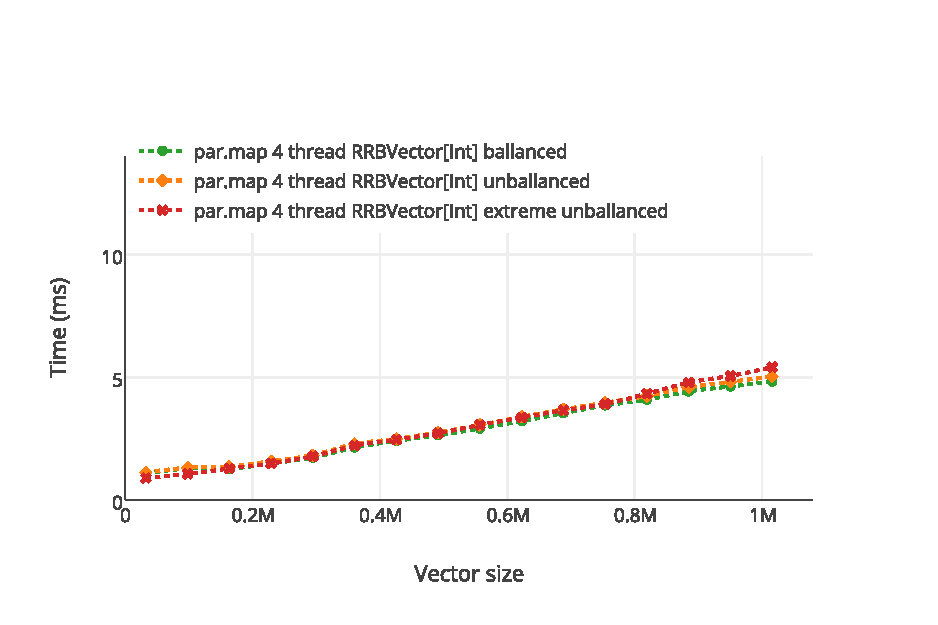
\includegraphics[width=0.49\textwidth]{Benchmarks/parmap_unbalanced_4.pdf}
  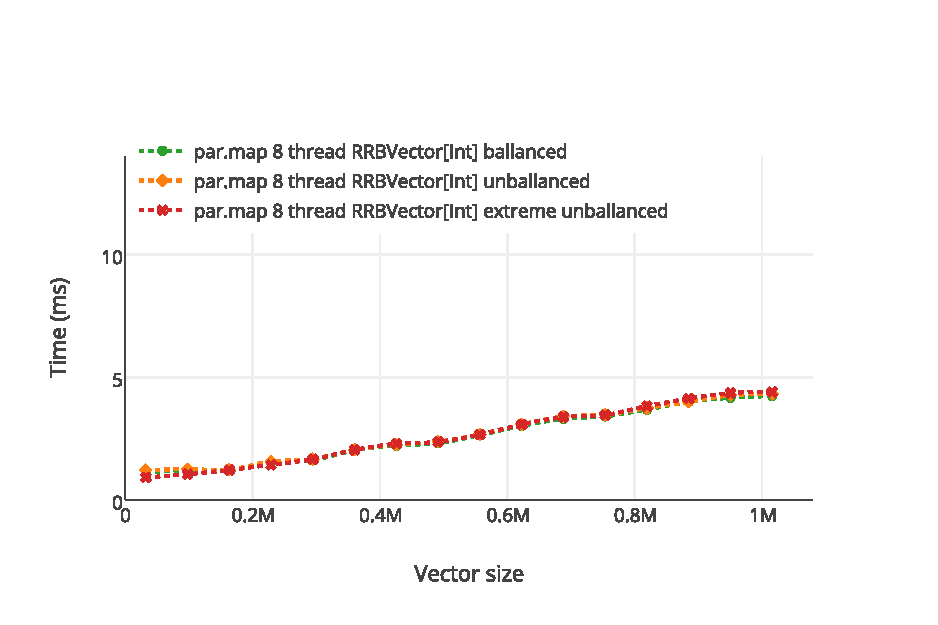
\includegraphics[width=0.49\textwidth]{Benchmarks/parmap_unbalanced_8.pdf}
  \label{ParallelUnbalancedBenchmarks}
  \caption{Benchmark on map and parallel map using the function (\textsc{x=>x}) to show the difference time used in the framework. This time represents the time spent in the splitters and combiners of the parallel collection.}
\end{figure}


%-----------------------------------
%	SUBSECTION Memory footprint
%-----------------------------------

\subsection{Memory footprint}
% describe the benchmark function
% compare expectation with results
% explain the upper bound
% explain apparently incoherent results
\color{red} TODO \color{black}

\begin{figure}[h!]
  \centering
  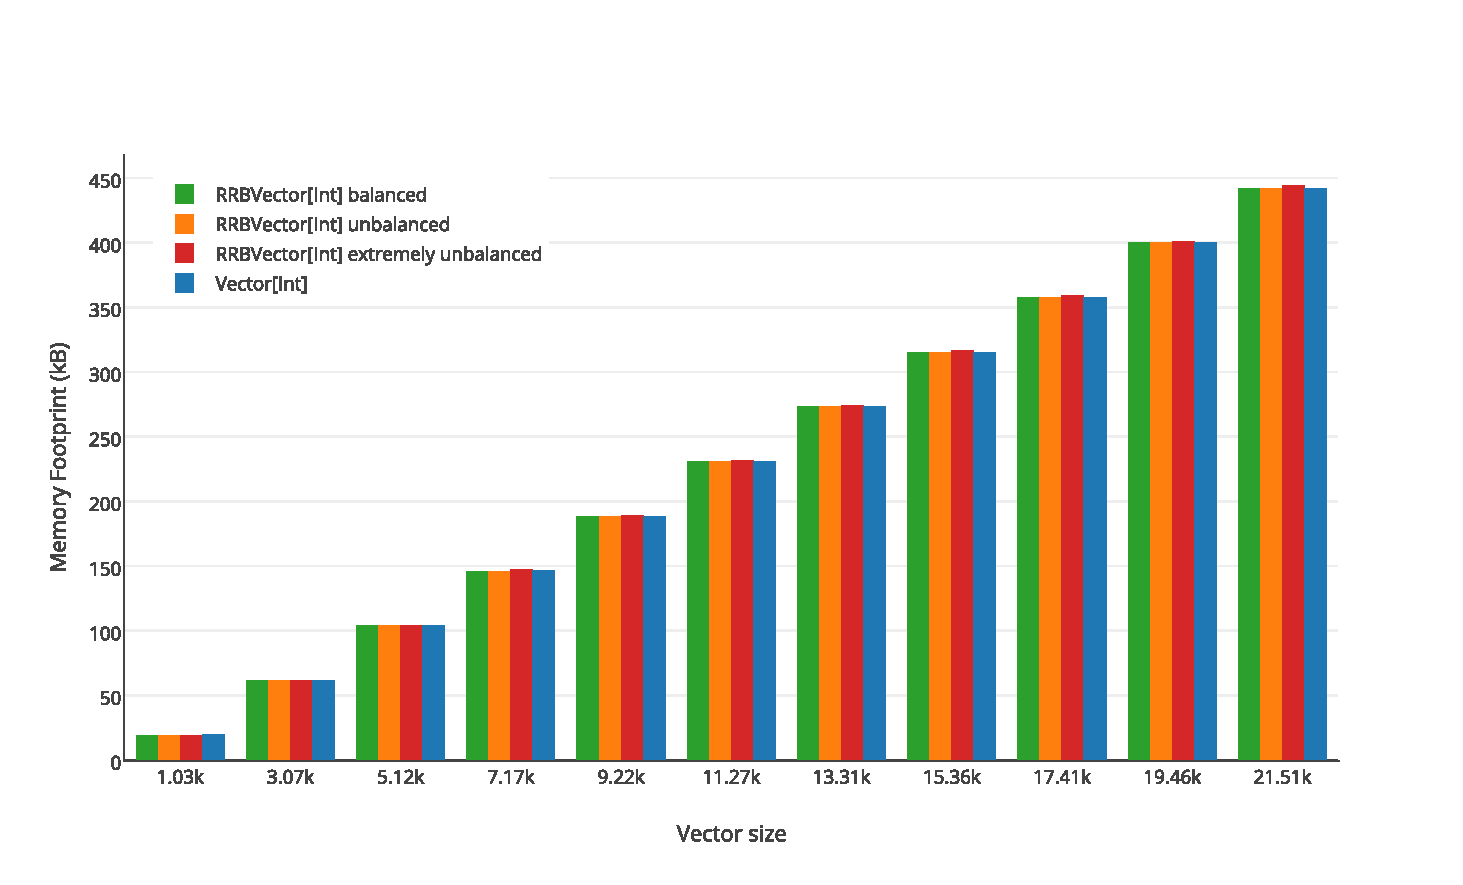
\includegraphics[width=\textwidth]{Benchmarks/Memory_3.pdf}
  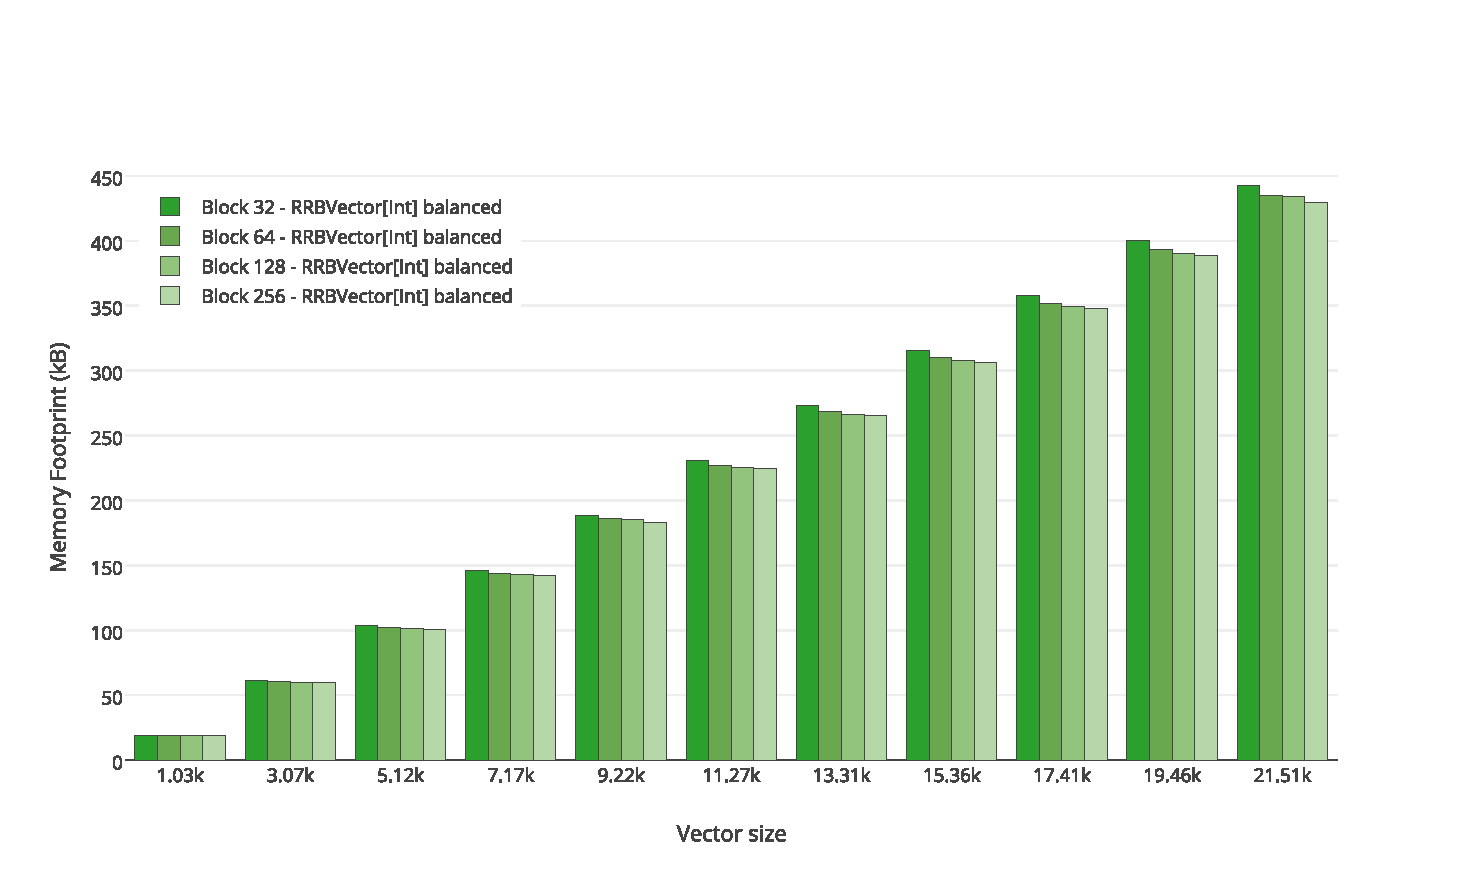
\includegraphics[width=\textwidth]{Benchmarks/Memory_blocks.pdf}
  \label{MemoryFootprints}
  \caption{Memory Footprint}
\end{figure}




I% Chapter Template

\chapter{Testing} % Main chapter title

\label{Testing} % Change X to a consecutive number; for referencing this chapter elsewhere, use \ref{ChapterX}

\lhead{Testing. \emph{Testing}} % Change X to a consecutive number; this is for the header on each page - perhaps a shortened title

%----------------------------------------------------------------------------------------
%	SECTION Teststing correctness
%----------------------------------------------------------------------------------------

\section{Teststing correctness}

%-----------------------------------
%	SUBSECTION Unit Tests
%-----------------------------------
\subsection{Unit tests}
% black box testing
% types of vector tested (balanced and different unbalanced vectors)
% pseudorandom set of differently unbalanced vectors
% comparing results of operations with other collections like lists
% use of tests suit on old Vector to check that tests are correct and coherent 
\color{red} TODO \color{black}

%-----------------------------------
%	SUBSECTION Invariant Assertions
%-----------------------------------
\subsection{Invariant Assertions}
% white box testing with assertions
% explain how the invariants of the whole rrb-tree can be checked using assertions
% list and describe assertions used
\color{red} TODO \color{black}


 
I% Chapter Template

\chapter{Related Work} % Main chapter title

\label{RelatedWork} % Change X to a consecutive number; for referencing this chapter elsewhere, use \ref{ChapterX}

\lhead{Related Work} % Change X to a consecutive number; this is for the header on each page - perhaps a shortened title

%----------------------------------------------------------------------------------------
%	SECTION RRB-Vectors in Clojure
%----------------------------------------------------------------------------------------

\section{RRB-Vectors in Clojure}

% Describe the improvements proposed with transience

% Describe fundamental difference between this transience and the display one.



 
I% Chapter Template

\chapter{Conclusions} % Main chapter title

\label{Conclusions} % Change X to a consecutive number; for referencing this chapter elsewhere, use \ref{ChapterX}

\lhead{Conclusions.} % Change X to a consecutive number; this is for the header on each page - perhaps a shortened title

%----------------------------------------------------------------------------------------
%	CONCLUSIONS
%----------------------------------------------------------------------------------------

 

%----------------------------------------------------------------------------------------
%	THESIS CONTENT - APPENDICES
%----------------------------------------------------------------------------------------

%\addtocontents{toc}{\vspace{2em}} % Add a gap in the Contents, for aesthetics

%\appendix % Cue to tell LaTeX that the following 'chapters' are Appendices

% Include the appendices of the thesis as separate files from the Appendices folder
% Uncomment the lines as you write the Appendices

%% Appendix A

\chapter{Appendix Title Here} % Main appendix title

\label{AppendixA} % For referencing this appendix elsewhere, use \ref{AppendixA}

\lhead{Appendix A. \emph{Appendix Title Here}} % This is for the header on each page - perhaps a shortened title

Write your Appendix content here.
%\input{Appendices/AppendixB}
%\input{Appendices/AppendixC}

%\addtocontents{toc}{\vspace{2em}} % Add a gap in the Contents, for aesthetics

%\backmatter

%----------------------------------------------------------------------------------------
%	BIBLIOGRAPHY
%----------------------------------------------------------------------------------------

\label{Bibliography}

\lhead{\emph{Bibliography}} % Change the page header to say "Bibliography"

\bibliographystyle{unsrtnat} % Use the "unsrtnat" BibTeX style for formatting the Bibliography

\bibliography{Bibliography} % The references (bibliography) information are stored in the file named "Bibliography.bib"

\end{document}